%\documentclass[12pt,draftcls]{ucdavisthesis}
\documentclass[12pt, nofigureslist, notableslist,twoside]{ucdavisthesis}

% PLEASE READ THE MANUAL - ucdavisthesis.pdf (in the package installation directory)

%%%%%%%%%%%%%%%%%%%%%%%%%%%%%%%%%%%%%%%%%%%%%%%%%%%%%%%%%%%%%%%%%%%%%%%%
%                                                                      %
%               LATEX COMMANDS FOR DOCUMENT SETUP                      %
%                                                                      %
%%%%%%%%%%%%%%%%%%%%%%%%%%%%%%%%%%%%%%%%%%%%%%%%%%%%%%%%%%%%%%%%%%%%%%%%

%\usepackage{bookmark}
\usepackage{lmodern}
\usepackage[us,nodayofweek,12hr]{datetime}
\usepackage{graphicx}
\usepackage{rotating}
\usepackage{subfigure}
\usepackage[none]{hyphenat}
\emergencystretch 3em
\usepackage[hyphens]{url}
\usepackage{hyperref}
\usepackage{amsmath}
\usepackage{enumitem}
\usepackage[capitalize]{cleveref}
\usepackage{multirow}
\usepackage{comment}
\usepackage{amsfonts}
\usepackage{courier}
\usepackage{amssymb}
\usepackage{rotating}
\usepackage{afterpage}
\usepackage{mathtools}
\newcommand\blankpage{%
    \null
    \thispagestyle{empty}%
    \addtocounter{page}{-1}%
    \newpage}

\hypersetup{%2
    pdfborder = {0 0 0}
}
\usepackage{bm}
\usepackage[parfill]{parskip}

\newcommand*{\figref}[2][]{%
  \hyperref[{fig:#2}]{%
    {Figure~\ref*{fig:#2}}%
    \ifx\\#1\\%
    \else
      \,#1%
    \fi
  }%
}

\newcommand*{\tabref}[2][]{%
  \hyperref[{tab:#2}]{%
    {Table~\ref*{tab:#2}}%
    \ifx\\#1\\%
    \else
      \,#1%
    \fi
  }%
}

\newcommand*{\eqnref}[2][]{%
  \hyperref[{eqn:#2}]{%
    {Equation~\ref*{eqn:#2}}%
    \ifx\\#1\\%
    \else
      \,#1%
    \fi
  }%
}

\newcommand*{\chapref}[2][]{%
  \hyperref[{chap:#2}]{%
    {Chapter~\ref*{chap:#2}}%
    \ifx\\#1\\%
    \else
      \,#1%
    \fi
  }%
}

\usepackage{accents}
\newlength{\dhatheight}
\newcommand{\doublehat}[1]{%
    \settoheight{\dhatheight}{\ensuremath{\hat{#1}}}%
    \addtolength{\dhatheight}{-0.35ex}%
    \hat{\vphantom{\rule{1pt}{\dhatheight}}%
    \smash{\hat{#1}}}}
        
\DeclareMathAlphabet\mathbfcal{OMS}{cmsy}{b}{n}   

%\addtolength{\parskip}{1\parskip}
%\usepackage[square,comma,numbers,sort&compress]{natbib}
%
% Different fonts to try (uncomment only fontenc and one font at a time)
% (you may need to install these first)
%\usepackage[T1]{fontenc} %enable fontenc package if using one of the fonts below
%\usepackage[adobe-utopia]{mathdesign}
%\usepackage{tgschola}
%\usepackage{tgbonum}
%\usepackage{tgpagella}
%\usepackage{tgtermes}
%\usepackage{fourier}
%\usepackage{fouriernc}
%\usepackage{kmath,kerkis}
%\usepackage{kpfonts}
%\usepackage[urw-garamond]{mathdesign}
%\usepackage[bitstream-charter]{mathdesign}
%\usepackage[sc]{mathpazo}
%\usepackage{mathptmx}
%\usepackage[varg]{txfonts}

\hyphenation{dis-ser-ta-tion blue-print man-u-script pre-par-ing} %add hyphenation rules for words TeX doesn't know

%\renewcommand{\rightmark}{\scriptsize A University of California Davis\ldots \hfill Rev.~\#1.0 \quad Compiled: \currenttime, \today}
% a fancier running header that can be used with draftcls options

%%%%%%%%%%%%%%%%%%%%%%%%%%%%%%%%%%%%%%%%%%%%%%%%%%%%%%%%%%%%%%%%%%%%%%%%
%                                                                      %
%        DOCUMENT SETUP AND INFORMATION FOR PRELIMINARY PAGES          %
%                                                                      %
%%%%%%%%%%%%%%%%%%%%%%%%%%%%%%%%%%%%%%%%%%%%%%%%%%%%%%%%%%%%%%%%%%%%%%%%

\title          {Robust Image-Based Modeling and Simulation in Biomechanics}
%Exact title of your thesis. Indicate italics where necessary by underlining or using italics. Please capitalize the first letter of each word that would normally be capitalized in a title.

\author         {Omar Mohamed Hafez}
%Your full name as it appears on University records. Do not use initials.

\authordegrees  {B.S. Civil Engineering (University of California, Davis) 2009 \\
                 M.S. Civil Engineering (University of California, Davis) 2010 \\
                 M.S. Applied Mathematics (University of California, Davis) 2012}
%Indicate your previous degrees conferred.

\officialmajor  {CIVIL AND ENVIRONMENTAL ENGINEERING}
%This is your official major as it appears on your University records.

\graduateprogram{Civil and Environmental Engineering}
%This is your official graduate program name. Used for UMI abstract.

\degreeyear     {2018}
% Indicate the year in which your degree will be officially conferred.

\degreemonth    {March}
% Indicate the month in which your degree will be officially conferred. Used for UMI abstract.

\committee{Mark Rashid}{N. Sukumar}{John Bolander}{}{}
% These are your committee members. The command accepts up to five committee members so be sure to have five sets of braces, even if there are empties.

%%%%%%%%%%%%%%%%%%%%%%%%%%%%%%%%%%%%%%%%%%%%%%%%%%%%%%%%%%%%%%%%%%%%%%%%

%\copyrightyear{2018}
%\nocopyright

%%%%%%%%%%%%%%%%%%%%%%%%%%%%%%%%%%%%%%%%%%%%%%%%%%%%%%%%%%%%%%%%%%%%%%%%

\dedication{\textsl{To Mama, Baba, and Asmaa}}
\intentional{This page intentionally left blank}
%%%%%%%%%%%%%%%%%%%%%%%%%%%%%%%%%%%%%%%%%%%%%%%%%%%%%%%%%%%%%%%%%%%%%%%%

\abstract{Image-based modeling and simulation has become an important analytic and predictive tool for patient-specific medical applications, including large-scale in-silico patient studies; optimized medical device design; and custom surgical guides and implants via additive manufacturing. The pipeline of steps for patient-specific modeling and simulation are: image acquisition, image segmentation, mesh generation, physics-based modeling and simulation, and finally clinical application. This research establishes a semi-automatic workflow for these steps, which includes a novel image-based meshing tool \textit{Shabaka}. The workflow is demonstrated in modeling the mechanics of a beating human heart based on magnetic resonance imaging (MRI) data.

Medical images are processed and segmented using thresholding, region-growing, and manual techniques. Watertight surface meshes are extracted from image masks using a novel Voronoi partitioning scheme. For scientific computing purposes, surface meshes are supplied either to tetrahedral meshing routines for conventional finite element approaches, or to a robust polyhedral mesh generation tool for a novel polyhedral finite element approach. The commercial polyhedral finite element code \textit{Celeris} is utilized, that retains most of the favorable properties of conventional finite element methods, while reducing the system size by up to an order of magnitude compared to conventional techniques for the same input surface.

In conjunction with the cardiac simulation code \textit{Cardioid} at Lawrence Livermore National Laboratory, the workflow is utilized to model the finite deformations of a beating heart. A quadratic tetrahedral mesh is generated from MRI data of the human heart ventricles. The constitutive law is comprised of an incompressible orthotropic hyperelastic stress response for the myocardium plus an electrical activation-dependent active stress for the muscle fibers. Muscle fiber orientations are generated using a rule-based approach. Electrical activation times are read from a coupled electrophysiology code. A lumped circulatory model is used to impose time-dependent ventricular volume constraints. Simulation results are presented. The same mechanics are also implemented for the polyhedral finite element mesh, and preliminary verification results are presented.

The tools developed and used for performing these image-based cardiac mechanics simulations make important improvements in the speed and robustness of image-based modeling techniques. As these tools continue to mature, so too does the promise for simulation to improve healthcare.}

%%%%%%%%%%%%%%%%%%%%%%%%%%%%%%%%%%%%%%%%%%%%%%%%%%%%%%%%%%%%%%%%%%%%%%%%

\acknowledgments{\noindent
Of the many lessons learned during this experience, one that tends to stick with me is that we are oftentimes more in control of our lives in the matters we think we are not, and less in control in the matters we think we are. The first part of that statement alludes to the hard work, self-reliance, and intrapersonal intelligence required to complete a PhD. The second part of that statement is an appreciation of just how much our successes in life depend on others. To that end, I humbly thank the following individuals, without whom I am utterly certain I would not have completed this degree:
 
I would first like to thank my advisor Professor Mark Rashid. I am forever grateful for his standard of excellence, precision of scientific communication, academic and emotional intelligence, and patience. I recall him telling me years ago ``you are not remembered for what you start, but for what you finish.'' I have kept those words of wisdom close to me ever since. There are few people over the course of my life I have learned more from than Professor Rashid.

My sincerest thanks to the Cardioid group for including me in their incredible work, in particular David Richards, Robert Blake, and Jean-Luc Fattebert at Lawrence Livermore National Laboratory, and Viatcheslav Gurev at IBM. Their mentorship and support provided me the opportunity to gain a much more complete perspective on my research, and opened opportunities for me I could have only dreamed of. I would also like to thank Andrew Baldwin and Alipasha Sadri at Celeris for their diligent work on my incessant feature requests in their software.

Many thanks to Professors Robert MacLeod, Jeffrey Weiss, and Ross Whitaker at the University of Utah for organizing and accepting me into their summer course on Image-Based Biomedical Modeling. It was easily one of the most intense, enjoyable, and memorable periods of time during my PhD.

I have many people to thank for providing me the financial support needed to complete this degree. I am forever indebted to Professor Mark Rashid and David Richards; the Krell Institute and the Computational Science Graduate Fellowship; Floyd and Mary Schwall; those in charge of the Eugene Cota Robles Fellowship; the UC Davis Department of Civil and Environmental Engineering; and Professors Sashi Kunnath, Amit Kanvinde, and John Bolander for giving me the means to accomplish my goals.
Financial support from DOE CSGF grant DE-FG02-97ER25308 is gratefully acknowledged. The work of LLNL authors was performed under the auspices of the U.S. Department of Energy by Lawrence Livermore National Laboratory under Contract DE-AC52-07NA27344.

Thank you to Professors John Bolander, N. Sukumar, and Yannis Dafalias for their guidance and mentorship over all these years dating back to my Master's Degree. Thank you to James St\"{o}lken and Ryan Vignes at Lawrence Livermore National Laboratory for their knowledge and wisdom during a period when I was first trying to fully understand what it meant to do good research.

A special thank you to the students I instructed in ENG 104. They injected an energy and enthusiasm in me in a way I think only a group of young students can. I would especially like to thank Bryan Zhao, who has inspired me to be a better teacher, a better researcher, and a better person.

Thank you to my office mates Steven Wopschall and Brian Giffin for giving me something to look forward to every day at the office. I will forever cherish the impact they have had on my life. Likewise, thank you to my roommate during the Image-Based Biomedical Modeling course, Brett Steineman, for whom I share the same sentiments.

Many thanks to Vincente Pericoli, Eric Chin, Subhajit Banerjee, and Alexandros Petalas for helping organize our student group, and thanks to Rose McCallen for her endless supply of enthusiasm, advice, and connections to help us get on our feet.

Thank you to my friends, among which there are too many to list here. Between lending an ear, providing advice, offering a couch to sleep on during my many visits to Livermore, or just bringing a smile to my face, I sincerely thank them all.

My love and thanks are extended to my mother, father, and brothers, who gave me the comfort and motivation to stay the course even through the most difficult times.

My deepest thanks to Asmaa Hassanein for being my rock, for helping me find my center again, and for believing in me.

Lastly, I thank God, for Whom I live my life.

I think we are all interconnected in ways we do not understand - I am grateful to be connected with all of these individuals, as well as those I have forgotten to mention, and those I did not even know I owed.
}
%%%%%%%%%%%%%%%%%%%%%%%%%%%%%%%%%%%%%%%%%%%%%%%%%%%%%%%%%%%%%%%%%%%%%%%%

% Each chapter can be in its own file for easier editing and brought in with the \include command.
% Then use the \includeonly command to speed compilation when working on a particular chapter.
%%% \includeonly{chap1}

%\includeonly{chap7-conclusions}

\begin{document}

\newcommand{\bibfont}{\singlespacing}
% need this command to keep single spacing in the bibliography when using natbib

\bibliographystyle{ieeetr}
%many other bibliography styles are available (IEEEtran, mla, etc.). Use one appropriate for your field.

\makeintropages %Processes/produces the preliminary pages

\chapter{Overview}
%

\textit{Image-based modeling and simulation}, also known as \textit{patient-specific modeling and simulation} or \textit{in-silico modeling and simulation}, is the process of performing computations based on imaging data to analyze and predict the physical behavior of biological tissues.

benefits

possibilities

FDA
VV40?

cite everyone doing it

Image-based modeling and simulation covers a broad spectrum of fields, including image processing, computational geometry, numerical methods, and biomechanics. The workflow entails: image processing and image segmentation, image-based mesh generation, physics-based modeling and simulation, and finally a 

Medical images will be assumed here to be 

nonlinear solid mechanics
finite element methods and their variants

For the electronic version of this document, images may be zoomed into for detail.

rectilinear grid of voxels, or three-dimensional pixels
\chapter{Medical Imaging and Image Segmentation}
%

The first steps in image-based modeling and simulation involve \textit{image acquisition}, \textit{image processing}, and \textit{image segmentation}. Several techniques are available to produce three-dimensional image data of an anatomical region of interest and are reviewed herein. State-of-the art image processing and image segmentation approaches are summarized in this section as well.

%%%%%%%%%%%%%%%%%%%%%%%%%%%%%%%%%%%%%%%%%%%%%%%
%%%%%%%%%%%%%%%%%%%%%%%%%%%%%%%%%%%%%%%%%%%%%%%
\section{Imaging Approaches}
\label{Imaging Approaches}

Medical imaging is the process of generating discrete image representations of biological tissues. Of the many imaging modalities found in clinical and research settings, the most prevalent are \textit{magnetic resonance imaging} (MRI) and \textit{x-ray computed tomography} (CT). Both approaches are \textit{tomographic} in that they produce a series of two-dimensional images representing thin slices through the region, that are subsequently combined to produce a three-dimensional volume representation \cite{larobina_murino_2014}. The data measured during acquisition are different for each modality, and thus the use case typically governs which technique is most appropriate. Images typically have resolutions on the order of millimeter or sub-millimeter resolution. Several other imaging techniques exist - some of which provide more information than do MRI and CT - and are briefly presented in this section as well. Finally, typical data storage and file formats are discussed.

\subsection{Magnetic Resonance Imaging}
\label{Magnetic Resonance Imaging}

Magnetic resonance imaging (MRI) is the process of generating images via the physical phenomenon of nuclear magnetic resonance (NMR), in which nuclei in a magnetic field absorb and re-emit electromagnetic radiation at their \textit{resonant frequency}~\cite{NMR}. Gradients in the magnetic field are used to encode the response at different locations in the region. MRI provides excellent soft tissue contrast, for tissues such as articular cartilage, bone marrow, muscle, ligaments, and gray and white matter in the brain. Unlike CT, it does not use any harmful ionizing radiation~\cite{waldman_campbell}. A brief description of the basic physics in acquiring an MRI follows.

A strong external magnet generates a magnetic field $B_0\bm{e}_z$ that is constant in time and space, within which the patient or object is placed. For most clinical applications, the strength of this field is 1.5 Tesla or 3 Tesla. The $z$ direction corresponds to the image slice thickness direction. Shim coils are used to correct or "shim" the magnetic field so as to ensure good field homogeneity, which results in a high-quality signal~\cite{jacobs_2007}. Dipole moments in the nuclei of certain elements align either in parallel or anti-parallel to the direction of the applied magnetic field, similarly to how a bar magnet orients itself in the presence of an external magnetic field~\cite{hendrick_1994}. The parallel orientation provides a slightly lower energy state than that for the anti-parallel orientation, and thus the dipole moments prefer to align with the direction of the applied magnetic field. Prior to applying the external magnetic field, the random orientation of the nuclear magnetic dipoles in the tissue produce a zero net magnetization. Following the imposition of a static magnetic field, a net magnetization of tissue $M_0\bm{e}_z$ is produced from the preferential alignment of dipoles. See \figref{mr1}.

Due to the prevalence of hydrogen in biological tissues - most notably in water and fat - MR imaging is typically based on the behavior of the nuclear magnetic dipole of hydrogen.

\begin{figure}[ht]
\centering
\subfigure[]{%
		\includegraphics[scale=0.33]{media/0-imaging/mr1a.png}
\label{fig:mr11}}
\subfigure[]{%
		\includegraphics[scale=0.33]{media/0-imaging/mr1b.png}
\label{fig:mr12}}
%
\caption{Net magnetization $M_0$ in a voxel of tissue (a) prior to, and (b) following the application of a static external magnetic field $B_0$~\cite{hendrick_1994}}
\label{fig:mr1}
\end{figure}

If the net magnetization is perturbed from pointing in the same direction of a magnetic field $B\bm{e}_z$, the new magnetization $M$ \textit{precesses} about the $z$ axis. The \textit{precessional frequency} or \textit{Larmor frequency} $\omega$ is defined by the following relationship:
\begin{equation}
\omega = \gamma B
\end{equation}
where the constant $\gamma$ is the \textit{gyromagnetic ratio}, which is 42.6 MHz/T for hydrogen. In MR imaging, the net magnetization is tipped away from the direction of $B_0$ by applying a radio-frequency (RF) pulse that oscillates exactly at the Larmor frequency. The precessing transverse magnetization produces a changing magnetic field, which induces an electric current and is recorded by the receiver coil. See \figref{mr2}.

\begin{figure}[ht]
\centering
\subfigure[]{%
		\includegraphics[scale=0.25]{media/0-imaging/mr2a.png}
\label{fig:mr21}}
\subfigure[]{%
		\includegraphics[scale=0.25]{media/0-imaging/mr2b.png}
\label{fig:mr22}}
\subfigure[]{%
		\includegraphics[scale=0.25]{media/0-imaging/mr2c.png}
\label{fig:mr23}}
%
\caption{Basic premise of MRI: (a) An external magnetic field $B_0$ causes net magnetization $M_0$ of a voxel of tissue pointing in the same direction as the applied field, (b) an RF pulse applied at the precessional frequency of hydrogen causes the magnetization vector to tilt from a longitudinal direction into the transverse plane, and (c) the amplitude, frequency, and phase of the time-varying signal from the transverse magnetization $M_{xy}$ is recorded~\cite{hendrick_1994}}
\label{fig:mr2}
\end{figure}

In order for the receiver coil to distinguish between different locations in the object, \textit{spatial localization} of the MR signal is achieved by applying linear magnetic field gradients in each of the three spatial directions. Namely, the new spatially varying magnetic field $B(\bm{x})\bm{e}_z$ (still pointing in $z$ direction), following the imposition of magnetic gradients, becomes:
\begin{equation}
B(\bm{x}) = B_0 + \bm{G}(t) \cdot \bm{x}
\label{eqn:gradient}
\end{equation}
The magnetic field gradient $\bm{G}(t) = (G_x, G_y, G_z)$ is applied in stages, to be discussed shortly. Multiplying \eqnref{gradient} by $\gamma$ yields:
\begin{equation}
\omega(\bm{x}) = \omega_0 + \bm{G}(t) \cdot \bm{x}
\label{eqn:freq}
\end{equation}
Thus, each RF signal oscillates at the appropriate frequency to excite and record information for each unique voxel in the image. Specifically, the magnetic gradient $G_z$ and corresponding RF pulse are first turned on to excite a particular slice (or section) of tissue. Excitation here refers to the perturbation of the net magnetization from the $z$ direction into the transverse plane. $G_z$ is referred to as the \textit{slice-selection gradient}. The resolution of the image in the $z$ direction may be increased by reducing the bandwidth of the RF pulse or increasing the strength of the applied gradient.

To resolve the selected section into voxels, gradients are applied separately in each of the two in-plane directions $x$ and $y$. The magnetic gradient $G_y$ is applied and removed following signal excitation and before signal measurement. While turned on, the gradient causes strips of hydrogen nuclei within the slice to precess at different speeds for a brief period of time. When the gradient is turned off, different strips maintain the same precessional frequency within the same slice, but a fixed phase difference now exists among them. $G_y$ is referred to as the \textit{phase-encoding gradient}. Finally, the magnetic gradient $G_x$ alters the resonant frequency along the $x$ direction. It separates each strip into voxels, each voxel resonating at a different frequency. $G_x$ is applied at the time of signal measurement and is referred to as the  \textit{frequency-encoding gradient} or the \textit{readout gradient}. The resolution of the in-plane image may be increased by increasing the number of pulse sequence acquisitions and subsequent measurements. See \figref{mr3} for a visual representation of these steps.

\begin{figure}[ht]
\centering
\subfigure[]{%
		\includegraphics[scale=0.21]{media/0-imaging/mr3a.png}
\label{fig:mr31}}
\subfigure[]{%
		\includegraphics[scale=0.21]{media/0-imaging/mr3b.png}
\label{fig:mr32}}
\subfigure[]{%
		\includegraphics[scale=0.21]{media/0-imaging/mr3c.png}
\label{fig:mr33}}
%
\caption{Visual representation of the process of spatial localization based on successive application of magnetic gradients: (a) slice-selection gradient, (b) phase-encoding gradient, and (c) frequency-encoding gradient~\cite{hendrick_1994}}
\label{fig:mr3}
\end{figure}

MRI signal intensity at a particular voxel typically depends on the proton density of the tissue (via the strength of the net magnetization $M_0$) and two \textit{relaxation times} T1 and T2 corresponding to the exponential decay of the perturbed net magnetization back to its original state following an RF pulse. Following a typical $90^{\circ}$ RF pulse, which maximizes the transverse magnetization $M_{xy}$, the relaxation times are defined as such:
\begin{equation}
M(t) = M_0(1 - e^{(-t/T1)})
\end{equation}
\begin{equation}
M_{xy}(t) = M_{xy}e^{(-t/T2)}
\end{equation}
The \textit{spin-lattice}, \textit{longitudinal}, or \textit{T1 recovery time} corresponds to the recovery of the longitudinal magnetization $M_0$. This reorientation is caused by the transfer of energy from the excited magnetic dipoles to the surrounding lattice of molecules. The \textit{transverse}, \textit{spin-spin}, or \textit{T2 recovery time} corresponds to neighboring precessing magnetic dipoles \textit{dephasing}. Dephasing is caused by different magnetic environments for different hydrogen nuclei within the same voxel as the transverse magnetization decays.

Tissue contrasts are created based on the strength and timing of the RF pulse; this is known as the \textit{MR sequence}. The parameters in MR pulse sequences weight the influence of proton density, T1, and T2 differently in the final MR signal. The most basic MR sequences are \textit{proton density} (PD), \textit{T1-weighted} (T1W), and \textit{T2-weighted} (T2W), each of which provide different tissue contrasts. The choice of an MR sequence will depend on the tissues and applications of interest of the scan. A number of references are available  \cite{nishimura_2010, brown_semelka_2003, webb_2003} for a more detailed description of T1, T2, the parameters of an MR sequence, and their relationship in creating tissue contrast.

For each voxel in a slice, the amplitude, phase, and frequency of the time-varying MR signal is recorded by the receiver coil in the \textit{frequency domain}, or what is known as \textit{k-space}. For each slice, the frequency domain is converted to the spatial domain (i.e., the two-dimensional image for a particular slice) via 2D inverse Fourier transform. The k-space of an image can be modified to identify artifacts, remove noise, and enhance contrast~\cite{imaios}. Please refer to the references in this section for more detail on k-space and its manipulations. Finally, each 2D image is combined to form a 3D grayscale image corresponding to the object scanned. The intensity at each voxel in the three-dimensional rectilinear grid is a weighted proton density. The value at each voxel can represent many different units of measure depending on the pulse sequence~\cite{beek_hoffman_2008}.

\subsection{X-Ray Computed Tomography}
\label{X-Ray Computed Tomography}

X-ray computed tomography (CT) is the process of generating images via the emission an x-ray beam source, and subsequently detecting the \textit{attenuation} of the x-ray beam through the various tissues in the patient or object. CT provides excellent contrast for bone, but is less suitable in measuring soft tissue contrast compared to MRI. Acquisition times are typically less than those for MRI, image resolutions are typically higher~\cite{pomeranz_2007}, and ionizing radiation from the x-ray beam must be carefully considered. The basic principles of image acquisition via CT technology ensues.

In CT, an x-ray beam source is emitted through the plane of a finite thickness cross section of the object~\cite{mahesh_2002}. The mean attenuation of the x-ray beam through each voxel within the slice is measured by a detector on the other side of the object. The attenuation data is reconstructed into a digital two-dimensional image. Once again, the set of 2D images is stacked together to form a 3D image representation of the region being scanned.

Attenuation measures the amount by which x-ray radiation is reduced in passing through material. For an inhomogeneous material, the attenuation along a particular ray line is expressed in the following relationship:
\begin{equation}
I= I_0e^{-\int\limits_{0}^{L}f(x,y) ds}
\label{eqn:init}
\end{equation}
where $I_0$ is the x-ray intensity emitted in front of the object, $I$ is the x-ray intensity received behind the object, $f(x,y)$ is the linear attenuation coefficient for the material at location $(x,y)$, and $L$ is the length over which the beam travels though the material, and $ds$ is the length of a differential cut along the ray. The variable $s$ is parameterized as a function of $x$ and $y$. In first generation CT machines, for a particular slice, the x-ray tube and detector were rigidly translated together across the subject as x-ray beams were emitted and recorded~(\figref{ct1}).

\begin{figure}[ht]
\centering
		\includegraphics[scale=0.3]{media/0-imaging/ct1.png}
%
\caption{CT arrangement for linear transverse scanning motion of x-ray tube and detector. ~\cite{goldman_2007}}
\label{fig:ct1}
\end{figure}

The x-ray beam path is referred to as a \textit{ray}. The set of rays and measurements made during the the translation is known as a \textit{view}. Several hundred rays are measured in a particular view. The assembly is then rotated about the axis perpendicular to the slice plane by a small increment and a new view is captured. Over a 1000 views are captured as the assembly is rotated through 360$^{\circ}$. Thus, the total number of measurements for a particular slice is the number of rays per view multiplied by the number of views, and is on the order of a million measurement per slice in modern CT machines. See \figref{ct2}.

\begin{figure}[ht]
\centering
		\includegraphics[scale=0.3]{media/0-imaging/ct2.png}
%
\caption{Measurement procedure for first-generation CT. Rays are emitted from the x-ray tube and the attenuated radiation is measured by the detector. The assembly is translated in increments to cover the span of the slice. The process is repeated as the assembly is rotated in increments through 360$^{\circ}$, in this example in 1$^{\circ}$ degree increments~\cite{goldman_2007}}
\label{fig:ct2}
\end{figure}

\textit{Image reconstruction} is the process of deriving the average attenuation coefficient values $f$ for each voxel in a slice from the attenuation measurements made by the x-ray detector. Attenuation increases with the density and atomic number of the tissues in the voxel. Rearranging~\eqnref{init} yields:
\begin{equation}
p(\xi, \theta) = -\ln(I/I_0) = \int\limits_{0}^{L}f(x,y) ds
\end{equation}
The function $p(\xi,\theta)$ is known as the \textit{Radon transform} of the attenuation function $f(x,y)$. The angle $\theta$ corresponds to the angle of rotation of the view, and $\xi$ corresponds to the position along the measured x-ray projection~(\figref{ct3}).

\begin{figure}[ht]
\centering
		\includegraphics[scale=0.3]{media/0-imaging/ct3.png}
%
\caption{Linear attenuation function $f(x,y)$ for a particular slice, and corresponding projection $p(\xi,\theta)$}
\label{fig:ct3}
\end{figure}

The function $p$ for each $\theta$ view is known as a \textit{projection} of the image $f$. The most popular image reconstruction technique is \textit{backprojection}, in which the function $f$ is backprojected from the projections $p$. Backprojection leads to a blurring of the original image, so the projected images are first filtered prior to backprojection. The technique is known as \textit{filtered backprojection}. It involves computing the Fourier transform of $p$, applying a ramp filter to avoid blurring, computing the inverse Fourier transform of the resulting function, and finally the inverse Radon transform to approximate $f(x,y)$. Filtered backprojection performs best in the presence of a large number of projections, which is the case in modern CT scanners. Please refer to \cite{chetih_2015} for a more detailed description of the procedure.

Finally, the value computed at each voxel is rescaled to produce the \textit{CT number} = $K (f_i - f_w)/f_w$, measured in \textit{Hounsfield units}. The value $f_i$ is the attenuation at a particular voxel, and the value $f_w$ is the attenuation of water. The attenuation coefficient of water is obtained during calibration of the machine. The scaling parameter $K$ is typically a value of 1000 in modern machines.

Improvements in acquisition times, spatial resolution, and image reconstruction times have been made in the last 45 years since the first-generation CT machine was introduced. These improvements mostly involve and increase in x-ray detectors, and more clever arrangements and motions of the x-ray beam and associated detector(s). Detailed descriptions of these improvements can be found in the references cited in this section.

\subsection{Additional Imaging Modalities}
\label{Other Imaging Modalities}

Several other popular imaging modalities exist. The discussion here will be restricted to a brief overview of \textit{ultrasound} (US), as well as some quantitative variations of MRI, CT, and US.

Ultrasound uses high-frequency sound pulses that are emitted from a hand-held ultrasound transducer~\cite{waldman_campbell}. The transducer is applied to the patient's skin through a coupling gel, and sound pulses are reflected back to the transducer from structures within the patient. The magnitude of the reflected sound, or \textit{echo} is converted into a 2D grayscale image. Images are acquired in real-time, and do not require any ionizing radiation. Ultrasound is most commonly used for imaging the abdominal and pelvic regions, as well as imaging the musculoskeletal system. When used to image the heart, ultrasound is referred to as \textit{echocardiography}. Three-dimensional ultrasound techniques have been gaining traction in recent decades, of which there are two varieties for 3D reconstruction: random or \textit{freehand scanning} which is based on free motion of the ultrasound transducer; and \textit{sequential scanning} where the ultrasound motion is predetermined in linear, fan-like or rotational patterns~\cite{valocik_2005, bruining_2000}.

Quantitative versions of the modalities discussed typically attempt to extract material property information in addition to only contrasting different tissues. \textit{Diffusion-tensor imaging} (DTMRI) is used to measure the anisotropy of tissues. Additional magnetic field gradients are applied repeatedly to create images that are sensitized to the diffusion of water in specific directions~\cite{o’donnell_westin_2011}. Least squares is employed to estimate the diffusivity tensor at each voxel. The diffusivity tensor may be used to visualize irregularities in the microstructure of the brain~\cite{alexander_lee_lazar_field_2007}, or to approximate cardiac muscle fiber orientations. \textit{Elastography} is the process of quantitatively imaging the mechanical properties of soft tissues \textit{in vivo}, and is performed using magnetic resonance and ultrasound techniques~\cite{zaleska_2014}. The process involves applying a stress or source of motion that deforms the tissue, imaging the tissue response, and finally processing the data to generate images (\textit{elastograms}) of tissue mechanical properties.~\cite{glaser_manduca_ehman_2012}.\textit{Quantitative computed tomography} (QCT) estimates bone mineral density from CT attenuation data by using a calibration phantom during image acquisition. This information can be used to inform heterogeneous material definitions in computational models of bone~\cite{knowles_2016}.

A more complete review of medical imaging technologies can be found in a number of texts~\cite{suetens_2017, webb_2003}.

\subsection{File Formats}
\label{Data Format-IMG}

Medical images are typically stored as a combination of a short \textit{header} followed by \textit{pixel data}. The header is typically stored in ASCII format and the pixel data is typically binary. They may be found in the same file or in separate ones. Pixel data is often stored either as a set of two-dimensional images representing each slice, or as a single block of information corresponding to the 3D volume. In either case, data is stored as a 1D array, from which the data can be unrolled based on the axis ordering specified in the header. The header provides metadata to allow software to read and store the image based on the pixel data. Namely, the header contains the matrix dimensions, image resolution, image origin, axis order, data type of the pixel data (i.e., unsigned char, int, etc.), endianness of the pixel data, and data compression encoding (e.g., raw, gzip, bzip2). Additional information may be provided as well, including patient data, image acquisition parameters (e.g., MRI pulse sequence), and date of acquisition. On the clinical side, DICOM (Digital Imaging and Communications in Medicine) files are by far the most popular format for storing medical images, due to it's extensive metadata including patient information and image acquisition protocol. On the research side, several formats are available, including MATLAB~\cite{MATLAB}, NRRD (Nearly Raw Raster Data)~\cite{nrrd}, NIfTI (Neuroimaging Informatics Technology Initiative)~\cite{nifti}, and Analyze~\cite{analyzedirect}. These file formats are different flavors of the general format described above. They are geared more towards image post-processing compared to DICOM, by way of less detailed metadata sections.


%%%%%%%%%%%%%%%%%%%%%%%%%%%%%%%%%%%%%%%%%%%%%%%
%%%%%%%%%%%%%%%%%%%%%%%%%%%%%%%%%%%%%%%%%%%%%%%
\section{Image Segmentation Approaches}
\label{Image Segmentation Approaches}

Arguably the most challenging task in the workflow is the subsequent image processing and \textit{segmenting} of the image of interest. \textit{Image segmentation} is the process of ... \figref{seg}. Contrast differences between neighboring tissues can be difficult to identify. \textit{Image processing} involves applying filters to the image to alter voxel intensity values, which can remove noise and emphasize features of the image so as to improve the performance of image segmentation algorithms.

\begin{figure}[ht]
\centering
\subfigure[]{%
		\includegraphics[scale=0.165]{media/1-seg3d/1-raw.png}
\label{fig:seg1}}
\subfigure[]{%
		\includegraphics[scale=0.165]{media/1-seg3d/2-seg.png}
\label{fig:seg2}}
%
\caption{(a) MRI of \textit{ex-vivo} human heart, and (b) resulting segmented image mask}
\label{fig:seg}
\end{figure}

The first step in preparing the image data for segmentation is \textit{resampling}. Images most often 

RESAMPLING: for isotropic resolution

Gaussian blur, mean filter, median filter.

\subsection{Review of Image Segmentation Approaches}
\label{Review of Image Segmentation Approaches}

\subsection{Thresholding Methods}
\label{Thresholding Methods}

\subsection{Region-Growing Methods}
\label{Region-Growing Methods}

\subsection{Neural Networks}
\label{Neural Networks}

\subsection{Manual Methods}
\label{Manual Methods}

\subsection{File Formats}
\label{Data Format-SEG}

\chapter{Image-Based Meshing}
%
%%%%%%%%%%%%%%%%%%%%%%%%%%%%%%%%%%%%%%%%%%%%%%%
%%%%%%%%%%%%%%%%%%%%%%%%%%%%%%%%%%%%%%%%%%%%%%%
\section{Image-Based Meshing Approaches}
\label{Image-Based Meshing Approaches}

%%%%%%%%%%%%%%%%%%%%%%%%%%%%%%%%%%%%%%%%%%%%%%%
%%%%%%%%%%%%%%%%%%%%%%%%%%%%%%%%%%%%%%%%%%%%%%%
\section{Surface Generation}
\label{Surface Generation}
also referred to as surface extraction

%%%%%%%%%%%%%%%%%%%%%%%%%%%%%%%%%%%%%%%%%%%%%%%
%%%%%%%%%%%%%%%%%%%%%%%%%%%%%%%%%%%%%%%%%%%%%%%
\subsection{Point Cloud Generation}
\label{Point Cloud Generation}

%%%%%%%%%%%%%%%%%%%%%%%%%%%%%%%%%%%%%%%%%%%%%%%
%%%%%%%%%%%%%%%%%%%%%%%%%%%%%%%%%%%%%%%%%%%%%%%
\subsection{Surface Reconstruction}
\label{Surface Reconstruction}

\subsubsection{Surface Reconstruction Approaches}
\label{Surface Reconstruction Approaches}

\subsubsection{Voronoi-Based Surface Reconstruction}
\label{Voronoi-Based Surface Reconstruction}

\begin{figure}[ht]
\centering
\subfigure[]{%
		
\includegraphics[scale=0.57]{media/2-shabaka/1-vor/dem1.png}
\label{fig:vor1}}
\subfigure[]{%
		\includegraphics[scale=0.57]{media/2-shabaka/1-vor/dem2.png}
\label{fig:vor2}}
\subfigure[]{%
		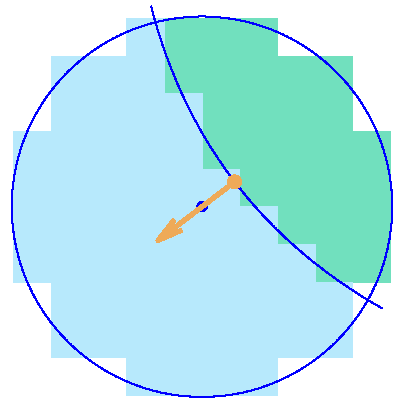
\includegraphics[scale=0.57]{media/2-shabaka/1-vor/dem3.png}
\label{fig:vor3}}
\subfigure[]{%
		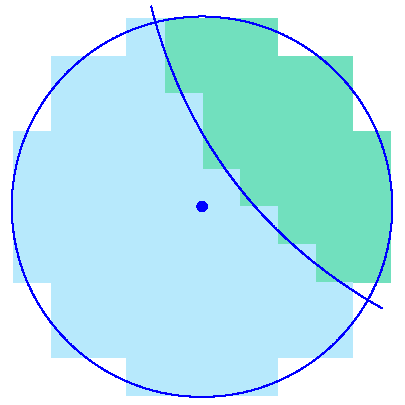
\includegraphics[scale=0.57]{media/2-shabaka/1-vor/dem4.png}
\label{fig:vor4}}
%
\caption{(a) Sample window of segmented image, (b) interface approximation, (c) point/normal placement, and d) Voronoi site placement}
\label{fig:vor}
\end{figure}

\begin{figure}[ht]
\centering
\subfigure[]{%
		\includegraphics[scale=0.083]{media/2-shabaka/3-clean-zoom/1-init-zoom.png}
\label{fig:cross1-1}}		
\subfigure[]{%
		\includegraphics[scale=0.083]{media/2-shabaka/3-clean-zoom/2-badfacets-zoom.png}
\label{fig:cross1-2}}		
\subfigure[]{%
		\includegraphics[scale=0.083]{media/2-shabaka/3-clean-zoom/3-badsegs-zoom.png}		
\label{fig:cross1-3}}					
\subfigure[]{%
		\includegraphics[scale=0.083]{media/2-shabaka/3-clean-zoom/4-fine-zoom.png}
\label{fig:cross1-4}}				
%
\caption{Clean-up of undesirable ``cross-talk'' facets for a surface patch: (a) initial surface following Voronoi-based surface reconstruction, (b) identification of ``cross-talk'' facets, (c) identification of edges to be collapsed, (d) final cleaned surface.}
\label{fig:cross1}
\end{figure}

\begin{figure}[ht]
\centering
\subfigure[]{%
		\includegraphics[scale=0.07]{media/2-shabaka/4-clean/1-init.png}
\label{fig:cross2-1}}		
\subfigure[]{%
		\includegraphics[scale=0.07]{media/2-shabaka/4-clean/2-badfacets.png}
\label{fig:cross2-2}}		
\subfigure[]{%
		\includegraphics[scale=0.07]{media/2-shabaka/4-clean/3-badsegs.png}	
\label{fig:cross2-3}}						
\subfigure[]{%
		\includegraphics[scale=0.07]{media/2-shabaka/4-clean/4-fine.png}		
\label{fig:cross2-4}}		
%
\caption{Clean-up of undesirable ``cross-talk'' facets for surface of \textit{ex-vivo} human heart: (a) initial surface following Voronoi-based surface reconstruction, (b) identification of ``cross-talk'' facets, (c) identification of edges to be collapsed, (d) final cleaned surface.}
\label{fig:cross2}
\end{figure}

\begin{figure}[ht!]
\centering
\subfigure[]{%
		\includegraphics[scale=0.092]{media/2-shabaka/2-surf/1-seg.png}
\label{fig:shabakaseq1}}
\subfigure[]{%
		\includegraphics[scale=0.092]{media/2-shabaka/2-surf/2-normals.png}
\label{fig:shabakaseq2}}
\subfigure[]{%
		\includegraphics[scale=0.092]{media/2-shabaka/2-surf/3-ptcloud.png}
\label{fig:shabakaseq3}}
\subfigure[]{%
		\includegraphics[scale=0.092]{media/2-shabaka/2-surf/4-finesurf.png}
\label{fig:shabakaseq4}}
\subfigure[]{%
		\includegraphics[scale=0.092]{media/2-shabaka/2-surf/5-surf.png}
\label{fig:shabakaseq5}}
%
\caption{(a) Segmented image, (b) point/normal placement, (c) oriented point cloud (normals not shown), c) cleaned surface mesh generated from Voronoi partition (edges not shown), and d) final decimated surface}
\label{fig:shabakaseq}
\end{figure}

\begin{figure}[ht!]
\centering
\vspace{2.5mm}
\includegraphics[width=1.0\textwidth]{media/2-shabaka/2-surf/6-showcase.png}
\caption{Suite of example surfaces generated from image data.}
\label{fig:showcase}
\end{figure}

\begin{figure}[ht!]
\centering
\vspace{2.5mm}
\includegraphics[width=1.0\textwidth]{media/2-shabaka/2-surf/7-shabaka.png}
\caption{Screenshot of Github repo}
\label{fig:github}
\end{figure}

%%%%%%%%%%%%%%%%%%%%%%%%%%%%%%%%%%%%%%%%%%%%%%%
%%%%%%%%%%%%%%%%%%%%%%%%%%%%%%%%%%%%%%%%%%%%%%%
\subsection{File Formats}
\label{File Formats-SURF}


\section{Mesh Generation}
%

%%%%%%%%%%%%%%%%%%%%%%%%%%%%%%%%%%%%%%%%%%%%%%%
%%%%%%%%%%%%%%%%%%%%%%%%%%%%%%%%%%%%%%%%%%%%%%%
\subsection{Hexahedral and Hex-Dominant Meshing}
\label{Hexahedral and Hex-Dominant Meshing}

%%%%%%%%%%%%%%%%%%%%%%%%%%%%%%%%%%%%%%%%%%%%%%%
%%%%%%%%%%%%%%%%%%%%%%%%%%%%%%%%%%%%%%%%%%%%%%%
\subsection{Tetrahedral Meshing}
\label{Tetrahedral Meshing}

%%%%%%%%%%%%%%%%%%%%%%%%%%%%%%%%%%%%%%%%%%%%%%%
%%%%%%%%%%%%%%%%%%%%%%%%%%%%%%%%%%%%%%%%%%%%%%%
\subsection{Polyhedral Meshing}
\label{Polyhedral Meshing}


\begin{figure}[ht]
\centering
\subfigure[]{%
		\includegraphics[scale=0.14]{media/4-cardioid/0-ventriclesurf.png}
\label{fig:tet1}}
\subfigure[]{%
		\includegraphics[scale=0.14]{media/4-cardioid/1-tet.png}
\label{fig:tet2}}
%
\caption{Bi-ventricular mesh: (a) surface mesh, and (b) clipped view of quadratic tetrahedral mesh used in Cardioid simulations}
\label{fig:tetmesh}
\end{figure}

\begin{figure}[ht]
\centering
\subfigure[]{%
		\includegraphics[scale=0.18]{media/3-celeris/1-brep.png}
\label{fig:cel1}}		
\subfigure[]{%
		\includegraphics[scale=0.18]{media/3-celeris/2-hex.png}
\label{fig:cel2}}		
\subfigure[]{%
		\includegraphics[scale=0.18]{media/3-celeris/3-pmesh.png}
\label{fig:cel3}}		
\subfigure[]{%
		\includegraphics[scale=0.18]{media/3-celeris/4-clip.png}
\label{fig:cel4}}	
\subfigure[]{%
		\includegraphics[scale=0.18]{media/3-celeris/5-color.png}
\label{fig:cel5}}			

\caption{Generation of polyhedral mesh: (a) input surface mesh, (b) bounding hex mesh,  (c) resulting polyhedral mesh, (d) clipped mesh, and (e) highlight of elements with cuboidal vs. general polyhedral shape.}
\label{fig:cel}
\end{figure}

\begin{figure}[ht]
\centering
\subfigure[]{%
		\includegraphics[scale=0.125]{media/3-celeris/zoom/zoom1.png}
\label{fig:zoom1}}		
\subfigure[]{%
		\includegraphics[scale=0.125]{media/3-celeris/zoom/zoom2.png}
\label{fig:zoom2}}		
\subfigure[]{%
		\includegraphics[scale=0.125]{media/3-celeris/zoom/zoom3.png}
\label{fig:zoom3}}		
\subfigure[]{%
		\includegraphics[scale=0.125]{media/3-celeris/zoom/zoom4.png}
\label{fig:zoom4}}	
\subfigure[]{%
		\includegraphics[scale=0.125]{media/3-celeris/zoom/zoom5.png}
\label{fig:zoom5}}		
\subfigure[]{%
		\includegraphics[scale=0.125]{media/3-celeris/zoom/zoom6.png}
\label{fig:zoom6}}	

\caption{Three example arbitrary polyhedral elements presented at different angles}
\label{fig:zoom}
\end{figure}

\begin{figure}[ht]
\centering
\includegraphics[width=1.0\textwidth]{media/3-celeris/7-suite.png}
\caption{Suite of polyhedral finite element meshes generated from image data \vspace{1cm}}
\label{fig:celsuite}
\end{figure}

%%%%%%%%%%%%%%%%%%%%%%%%%%%%%%%%%%%%%%%%%%%%%%%
%%%%%%%%%%%%%%%%%%%%%%%%%%%%%%%%%%%%%%%%%%%%%%%
\subsection{File Formats}
\label{File Formats-MESH}


\section{Shabaka: A Free Image-Based Meshing Tool}
\chapter{Physics-Based Modeling and Simulation}
\label{chap:4}
%
%%%%%%%%%%%%%%%%%%%%%%%%%%%%%%%%%%%%%%%%%%%%%%%
%%%%%%%%%%%%%%%%%%%%%%%%%%%%%%%%%%%%%%%%%%%%%%%
\section{Continuum Mechanics}
\label{Continuum Mechanics}

stress measures

%%%%%%%%%%%%%%%%%%%%%%%%%%%%%%%%%%%%%%%%%%%%%%%
%%%%%%%%%%%%%%%%%%%%%%%%%%%%%%%%%%%%%%%%%%%%%%%
\section{The Finite Element Method}
\label{The Finite Element Method}

element quality
%%%%%%%%%%%%%%%%%%%%%%%%%%%%%%%%%%%%%%%%%%%%%%%
%%%%%%%%%%%%%%%%%%%%%%%%%%%%%%%%%%%%%%%%%%%%%%%
\section{The Partitioned Element Method}
\label{The Partitioned Element Method}

%%%%%%%%%%%%%%%%%%%%%%%%%%%%%%%%%%%%%%%%%%%%%%%
%%%%%%%%%%%%%%%%%%%%%%%%%%%%%%%%%%%%%%%%%%%%%%%
\section{Incremental Kinematics}
\label{Incremental Kinematics}

%%%%%%%%%%%%%%%%%%%%%%%%%%%%%%%%%%%%%%%%%%%%%%%
%%%%%%%%%%%%%%%%%%%%%%%%%%%%%%%%%%%%%%%%%%%%%%%
\section{Hyperelastic Materials}
\label{Hyperelastic Materials}

%%%%%%%%%%%%%%%%%%%%%%%%%%%%%%%%%%%%%%%%%%%%%%%%%%%%%%%%%%%%%%%%%%%%%%%%%%%%%%%%%%%%%%%%%%%%%%%%%%%%%%%%
%%%%%%%%%%%%%%%%%%%%%%%%%%%%%%%%%%%%%%%%%%%%%%%%%%%%%%%%%%%%%%%%%%%%%%%%%%%%%%%%%%%%%%%%%%%%%%%%%%%%%%%%

\chapter{Application: Cardiac Mechanics}
\label{chap:5}
%
Provided the image-based meshing workflow fully developed in~\chapref{3}, together with the finite element approaches established in~\chapref{4}, the entire image-based modeling and simulation pipeline is demonstrated through modeling the mechanical behavior of a beating human heart. Cardiac mechanics is a good testbed for the particular image-based modeling and simulation workflow described because: 1) the application only involves binary image masks, 2) the exact geometry does not grossly affect results since contact modeling is not included, and 3) the use of simulation in this field arguably has the potential to save and improve more lives than any other biomechanics application area.

This chapter introduces and motivates the task of modeling the human heart. The essential components to computational cardiac mechanics are described for an implementation using conventional finite elements, and  simulation results are presented. Finally, the details of implementing the same mechanics into the polyhedral code \textit{Celeris} are discussed, along with verification results.

\section{Introduction}

A brief overview of the anatomy and function of the heart will be presented, followed by a survey of approaches found in the literature.

\subsection{Anatomy and Function of the Heart}
The heart consists of four chambers: the \textit{left ventricle} (LV), \textit{right ventricle} (RV), \textit{left atria} (LA), and \textit{right atria} (RA) (See~\figref{anatomy}). The \textit{septum} is the tissue wall that separates the LV and RV. The thinner-walled atria act as blood reservoirs for the ventricles, which are predominantly responsible for the pumping function. The entire heart is encompassed by a fibrous sac known as the \textit{pericardium}, which resists rapid increases in cardiac size. The primary function of the heart is to pump blood throughout the body, delivering nutrients and removing waste from each organ~\cite{holzapfel_2009}. Cyclic pumping of the heart arises from the interaction of its electrical and mechanical function. Namely, the electrical activation of cardiac muscle fibers causes an excitation and contraction of tissue that drives the motion of the organ. Myocardial tissue consists of discrete muscle fiber bundles that exhibit orthotropic material behavior. For a more detailed description of the macro and microstructural properties of the heart, refer to Holzapfel \textit{et al.}~\cite{holzapfel_2009} and Hunter~\cite{holzapfel_2009} 

\begin{figure}[htbp!]
\centering
\includegraphics[width=1.0\textwidth]{media/anatomy.png}
\caption{Longitudinal cross-section of the human heart~\cite{katz_2015}}
\label{fig:anatomy}
\end{figure}

\subsection{Related Work}
Cardiovascular disease is the leading cause of death and disability, accounting for about 40$\%$ of all human mortality~\cite{genet_2015}. Heart failure is one of the most common, costly, and deadly medical conditions, affecting more than 25 million people worldwide~\cite{mann_2015}. Better understanding the nuanced electrical and mechanical behavior of normal and pathological hearts is an important step in improving treatment for heart disease. The complexity of the mechanisms of interest, time and cost savings offered by simulation, and the high sensitivity to various patient-specific parameters make \textit{in silico} modeling an important tool in addressing heart disease.

Indeed, cardiac mechanics is one of the most mature fields in computational biomechanics. Several well-known groups have advanced the field using a variety of approaches with respect to the geometry and meshing. \textit{The Living Heart Project}~\cite{genet_2015, baillargeon_2014} has arguably gained the most traction in advancing the understanding of whole-heart cardiac mechanics through simulation, albeit using linear tetrahedra for an artificial heart geometry not generated from medical imaging. Augustin \textit{et al.}~\cite{augustin_2016} also used linear tetrahedral finite elements, meshed from considerably smoothed surfaces originating from MRI data. Pleny of informative research still only models simplified geometries of the left ventricle~\cite{guccione_2005, sack_2016}, in conjunction even with cubic Hermite finite elements~\cite{mcculloch_2000}. Generally speaking, though, most modern approaches generate either bi-ventricular models (i.e., left and right ventricles) or whole heart models that include the atria and potentially other geometric structures.

Gurev \textit{et al.}~\cite{gurev_2015} performed mechanical simulations on a quadratic hex-dominant mixed element mesh of the human heart ventricles, whose work forms the basis for the cardiac mechanics explorations detailed in this chapter. The review article by Trayanova \textit{et al.}~\cite{trayanova_2011} provides an excellent summary of the various components involved in ventricular electromechanical modeling, many of which are discussed in this chapter.

\section[Demonstration using Conventional Finite Elements]{Demonstration using Conventional Finite \\ Elements}

The key features of \textit{Cardioid}~\cite{richards_2013, gurev_2015} will be highlighted, as is relevant to image-based cardiac mechanics modeling. Cardioid is a highly efficient and scalable code at Lawrence Livermore National Laboratory that utilizes high performance computing for modeling the electromechanics of cardiac arrhythmia. The code is used here to demonstrate the image-based modeling and simulation pipeline using conventional finite element methods.

%%%%%%%%%%%%%%%%%%%%%%%%%%%%%%%%%%%%%%%%%%%%%%%
%%%%%%%%%%%%%%%%%%%%%%%%%%%%%%%%%%%%%%%%%%%%%%%
\subsection{Methods}
\label{Methods}

In Cardioid, the body is assumed to undergo quasi-static finite deformations, body forces are assumed negligible, and the stress measure of interest is the second Piola-Kirchoff stress $\bm{S}$. Thus, balance of linear momentum reduces to the following equation:
\begin{equation}
(F_{ik}S_{kj}),_{j} = 0
\end{equation}

In order to fully define and solve these equations, the following are specified: the mesh, constitutive update, muscle fiber orientation, solution-dependent pressure boundary conditions, and the finite element solver. Each consideration will be described in turn.

%%%%%%%%%%%%%%%%%%%%%%%%%%%%%%%%%%%%%%%%%%%%%%%
%%%%%%%%%%%%%%%%%%%%%%%%%%%%%%%%%%%%%%%%%%%%%%%
\subsubsection{Mesh Generation}
\label{Mesh Generation}

A bi-ventricular mesh is generated using the procedures described in~\chapref{2} and \chapref{3}. Namely, an MRI of an \textit{ex vivo} human heart from the CardioVascular Research~\cite{cvgg} is segmented using the software Seg3D. Since the ventricles are most responsible for the pumping action, image segmentation is restricted to those geometric structures. A threshold segmentation is used as the initial seed to Seg3D's level set segmentation tool. Additional tools to \textit{fill holes} and \textit{dilate-erode} the image mask are utilized before a final sweep of manual paintbrushing is employed. Following careful manual inspection, the final image mask is input to Shabaka to generate a high quality surface of the heart ventricles with a total of 50k points. Tetgen is invoked to produce a tetrahedral mesh that honors the input surface and attempts to produce high quality tetrahedra for the purposes of finite element simulations. A maximum element volume of 2 \textit{mm$^3$} was imposed. Again, quadratic tetrahedral elements are chosen in favor of linear elements to avoid volumetric locking and/or impracticably fine meshes. The surface and volume meshes are shown in \figref{tetmesh} - the final quadratc tetrahedral mesh has 374k elements and 595k nodes.

%%%%%%%%%%%%%%%%%%%%%%%%%%%%%%%%%%%%%%%%%%%%%%%
%%%%%%%%%%%%%%%%%%%%%%%%%%%%%%%%%%%%%%%%%%%%%%%
\subsubsection{Material Model}
\label{Material Model}

The cardiac tissue is assumed to exhibit an additive stress decomposition, such that $\bm{S} = \bm{S}_p + \bm{S}_a$ at any point in the model. The \textit{active stress} $\bm{S}_a$ represents the stress induced through active contraction of muscle fibers, and the \textit{passive stress} $\bm{S}_p$ is the stress experienced by the surrounding tissue.

\textbf{Passive Stress}

The passive response of the cardiac tissue is characterized by an incompressible, transversely isotropic constitutive law by Usyk~\textit{et al.}~\cite{usyk_2002}. The strain energy density functional is given by:
\begin{gather}
W(\bm{C}) = \frac{C}{2}\left(e^Q -1\right) \\
Q = b_{ff} E^2_{ff} + b_{ss} E^2_{ss} + b_{nn} E^2_{nn} + b_{fs}\left(E^2_{fs} + E^2_{sf}\right) + b_{fn}\left(E^2_{fn} + E^2_{nf}\right) + b_{ns}\left(E^2_{ns} + E^2_{sn}\right)
\label{eqn:usyk}
\end{gather}
where $\bm{E}$ is the Green-Lagrange strain tensor expressed in a local orthonormal coordinate system with axes parallel to the local fiber, sheet, and sheet-normal $(f,s,n)$ directions, $\bm{E} = \frac{1}{2}(\bm{C} - \bm{I})$, and $C$, $b_{ff}$, $b_{ss}$, $b_{nn}$, $b_{fs}$, $b_{fn}$, and $b_{ns}$ are material parameters.

Incompressibility is fully enforced by solving for pressure unknowns as Lagrange multipliers in addition to nodal unknowns. In order to use the constitutive law in a fully incompressible context, the deviatoric and volumetric portions of the strain energy are separated as is done by Weiss~\textit{et al.}~\cite{weiss_1996}. Rather than defining the passive stress as simply $\bm{S}_p = \frac{\partial W}{\partial \bm{E}}$, the passive stress becomes:
\begin{equation}
\bm{S}_p= 2\frac{\partial{\tilde{W}(\tilde{\bm{C}})}}{\partial{\bm{C}}} - pJ\bm{C}^{-1}
\end{equation}
where $\tilde{W}(\tilde{\bm{C}})$ is the deviatoric component of the strain energy functional, $J = \text{det}(\bm{F})$, and $\tilde{\bm{C}} = J^{-2/3}\bm{C}$. More details regarding the enforcement of incompressibility can be found in Gurev \textit{et al.}~\cite{gurev_2015} and Weiss~\textit{et al.}~\cite{weiss_1996}.

\textbf{Active Stress}

The active stress is defined as :
\begin{equation}
\bm{S}_a = \sigma_a \bm{f} \bm{f}^{T}
\label{eqn:active}
\end{equation}
where $\bm{f}$ is the muscle fiber direction and ${\sigma_a}$ is the scalar active tension induced in the fiber direction. The vector $\bm{f}$ here may refer to the fiber orientation either in the reference configuration or the current configuration - within Cardioid it refers to the direction in the reference configuration.

The model by Lumens \textit{et al.}~\cite{lumens_2009} is used to determine the active tension $\sigma_a$ in the following manner:
\begin{align}
\frac{d\bm{w}}{dt} = \bm{q}(\bm{w}; t_a, \lambda) \\
\sigma_a \equiv \sigma_a(\bm{w}; t_a, \lambda)
\end{align}
The scalar active tension depends on the state variables $\bm{w}$ of the muscle cells, the time $t_a$ at which the muscle cells electrically activate, and the muscle fiber stretch $\lambda$ in the direction of $\bm{f}$. Specifically, the fiber stretch is defined as $\lambda = (\bm{f}\bm{C}\bm{f}^T)^{1/2}$. The state variables are updated using a forward Euler scheme within the constitutive update. Further details on the state variables $\bm{w}$ and the way in which they are updated via $\bm{q}$ can be found in the work by Lumens~\textit{et al.}~\cite{lumens_2009}.

The activation time $t_a$ at each integration point is gathered from the results of the electrophysiology portion of the Cardioid code~\cite{richards_2013}. Specifically, an electrostatics problem is solved numerically for time-varying voltages, and the the activation time is determined based on when the voltage at each location passes a certain threshold. A one-way coupling is thus imposed, in which the mechanics code depends on the electrophysiology results, but not vice versa. A fixed beat duration $t_b$ is assumed, such that the myofilament model excites and contracts for the $n$th beat at time $nt_b + t_a$. Activation times are stored in the mechanics code as a field variable (see \figref{supp1}).

\begin{sidewaysfigure}[htbp!]
\centering
\subfigure[]{%
		\includegraphics[scale=0.11]{media/4-cardioid/22-activationtime.png}
\label{fig:supp1}}
\subfigure[]{%
		\includegraphics[scale=0.11]{media/4-cardioid/3-fibers.png}
\label{fig:supp2}}
\subfigure[]{%
		\includegraphics[scale=0.11]{media/4-cardioid/4-tagged.png}
\label{fig:supp3}}
%
\caption{Mechanics modeling considerations: (a) electrical activation times, (b) muscle fiber orientations, and c) surface tagging and prescription of corresponding boundary conditions.}
\label{fig:supp}
\end{sidewaysfigure}

\textbf{Fiber Generation}

Both the passive and active portions of the constitutive model depend on the muscle fiber orientation. Fiber orientations may be generated directly from DTMRI data, but that process requires denoising, smoothing, and interpolating tensor datasets, which can lead to unsatisfactory results. Additionally, DTMRI data is more expensive to acquire, and may not always be available. The Cardioid fiber generation code opts for the more popular \textit{rule-based approach}, in which fiber orientations are artificially generated based on the input mesh to mimic the actual muscle fiber orientations. The code utilizes the algorithm by Bayer \textit{et al.}~\cite{bayer_2012}, which involves solving Laplace's equation $\nabla^2\phi = 0$ four times, each with different Dirichlet boundary conditions (see~\figref{bayer}).

\begin{figure}[ht]
\centering
		\includegraphics[scale=0.3]{media/bayer.png}
\caption{Boundary conditions and resulting scalar solutions to Laplace's equation in Bayer \textit{et al.}~\cite{bayer_2012}. The gradients of the solutions are used to construct the rule-based fiber orientations}
\label{fig:bayer}
\end{figure}

The gradients of these solutions inform the construction of orthotropic fiber orientations at each solution point. Fiber orientations are then interpolated at the junctions between the LV, RV, and septum to ensure that the fiber direction changes smoothly and continuously throughout the entire myocardium. The details by which the gradients are used to construct the fiber orientations and by which orientations are interpolated are explained in Bayer~\textit{et al.}~\cite{bayer_2012}. The Laplace solves are performed using the highly parallelized finite element code \textit{MFEM}~\cite{mfem-library} on the same input quadratic tetrahedral mesh to be used for the mechanics simulation. The algorithm performs robustly for various geometries and compares well with fiber orientations generated directly from DTMRI data. The computed fiber orientations for the mesh of interest are shown in \figref{supp2}.

%%%%%%%%%%%%%%%%%%%%%%%%%%%%%%%%%%%%%%%%%%%%%%%
%%%%%%%%%%%%%%%%%%%%%%%%%%%%%%%%%%%%%%%%%%%%%%%
\subsubsection{Boundary Conditions}
\label{Boundary Conditions}

Fluid flow and fluid-structure interaction are not yet implemented in the Cardioid code, so ventricular volume constraints are imposed to mimic the effect of blood flow. The volumes of the ventricle cavities are calculated based on a lumped circulatory model by Kerckhoffs \textit{et al.}~\cite{kerckhoffs_2006}, which are in turn used to determine the time-varying, solution-dependent pressure boundary conditions.

A system of coupled ODEs describing the time evolution of the left ventricle volume $V_{LV}$ and the right ventricle volume $V_{RV}$ for the circulatory model can be written in the form:
\begin{align}
\frac{d\bm{w}_{c}}{dt} = \bm{q}_c(\bm{w}_c, p_{LV}, p_{RV}; t) \\
\frac{dV_{LV}}{dt} = g_{LV}(p_{LV}, \bm{w}_c; t) \\
\frac{dV_{RV}}{dt} = g_{RV}(p_{RV}, \bm{w}_c; t)
\end{align}
where $\bm{w}_c$ is the vector of state variables for the circulatory model, $p_{LV}$ and $p_{RV}$ are the pressures inside the left and right ventricles, and $\frac{dV_{LV}}{dt}$ and $\frac{dV_{RV}}{dt}$ represent the change in blood volume in each of the ventricles. The right hand side functions $\bm{q}_c$, $g_{LV}$, and $g_{RV}$ are described in detail in Kerckhoffs~\textit{et al.}~\cite{kerckhoffs_2006}. This paradigm assumes both that the blood is an incompressible fluid, and that the pressure is spatially uniform within each ventricle. For each time step, the ventricular volumes are calculated from the circulatory model and imposed as constraints on the finite element mesh to determine the corresponding ventricular pressures. The details by which the pressures are computed from the volume constraint are detailed in Gurev~\textit{et al.}~\cite{gurev_2015}. The lumped circulatory model is shown in~\figref{bcs}.
\begin{figure}[ht]
\centering
		\includegraphics[scale=0.3]{media/bcs.png}
\caption{Lumped circulatory model of Kerckhoffs \textit{et al.}~\cite{kerckhoffs_2006}. Variables shown in the schematic are parameters in the coupled system of ODEs, which are solved to obtain ventricular volumes at each time step.}
\label{fig:bcs}
\end{figure}

In order to avoid highly nonlinear solutions at the start of the simulation, initial pressures are applied linearly in the first 100 ms prior to ``turning on'' the active contraction and ventricular boundary conditions. The first 100 ms may be viewed as the period in which a \textit{residual stress} is applied.

Displacement boundary conditions are enforced such that the base of the heart is not allowed to move out of plane, and that a strip of the epicardium near the base experiences zero displacements in all directions. In order to enforce these displacement and pressure BCs, the appropriate surfaces must be identified. Identification of the base, epicardium, left ventricle, and right ventricle is a necessary intermediate step in generating fiber directions, so those boundary condition tags are available following execution of the fiber generation code (see~\figref{supp3}).

%%%%%%%%%%%%%%%%%%%%%%%%%%%%%%%%%%%%%%%%%%%%%%%
%%%%%%%%%%%%%%%%%%%%%%%%%%%%%%%%%%%%%%%%%%%%%%%
\subsubsection{Solver}
\label{Solver}

The quadratic tetrahedral mesh described previously is used together with the material model and boundary conditions to perform conventional finite element simulations in Cardioid. Cardioid employs a modified version of the freely available finite element library \textit{oomph-lib}~\cite{oomph}.

Because Cardioid uses an implicit mechanics approach, a linear system must be solved for each time step for incremental nodal unknowns. In the interest of solving problems with fine discretizations, Gurev \textit{et al.} avoid direct solvers of the linear system in Cardioid due to their poor scalability. Instead they employ a Krylov subspace iterative solver, which is more suitable for large scalable problems. The existence of active contraction creates saddle-points in the linear system that are addressed with a novel preconditioner. The details of the iterative solver may be found in Gurev \textit{et al.}~\cite{gurev_2015}.

The simulation was performed on the \textit{Surface} computing platform at Lawrence Livermore National Laboratory. The Moab schedule manager was used to submit the job, which was run on 50 nodes with 16 cores per node, for a total of 800 processes. With an assumed beat duration of 1000 $ms$ for a healthy human heart (i.e., 60 beats per minute), the simulation was run to a time of 5100 ms with a $\Delta t = 1$ $ms$ time increment. The simulation completed roughly one heartbeat per 24 hours of wall clock time. As mentioned, the first 100 ms are used to linearly apply the initial pressures for the simulation. The first beat is discarded as the heart reaches a dynamic steady state, and thus four full beats of a healthy human heart are extracted from the results.

%%%%%%%%%%%%%%%%%%%%%%%%%%%%%%%%%%%%%%%%%%%%%%%
%%%%%%%%%%%%%%%%%%%%%%%%%%%%%%%%%%%%%%%%%%%%%%%
\subsection{Results}
\label{Results}

Simulation results are shown in \figref{pv} and~\figref{snaps}. \figref{pv1} is known as a \textit{P-V loop} of the left ventricle, and \figref{pv2} is a time history plot of the pressures in the left and right ventricles. \figref{pv1} demonstrates the four stages of the cardiac cycle: 1) \textit{isovolumetric contraction} from label a to b, 2) \textit{ventricular ejection} of blood from label b to c, 3) \textit{isovolumetric relaxation} from label c to d, and 4) \textit{ventricular filling} from label d to a. Isovolumetric contraction and ventricular ejection comprise what is known as \textit{systole}, during which the ventricles are contracting. Isovolumetric relaxation and ventricular filling are known as \textit{diastole}, during which the ventricles are relaxing. The labels in \figref{pv1} correspond to the panels in~\figref{snaps} showing the deformed mesh with an overlay of fiber stretch $\lambda$. During a cycle, fiber stretch ranges from 0.6 to 1.4, certainly justifying the finite deformation approach. The results closely match those in Gurev~\textit{et al.}~\cite{gurev_2015}, in which a different heart geometry and electrophysiology is used. The full video of four heartbeats played at one quarter speed may be viewed at \href{http://youtu.be/RtQKEjdR4MU}{{\url{http://youtu.be/RtQKEjdR4MU}}}.

In the process of performing simulations, the workflow for generating the mesh; generating fiber orientations; running the electrophysiology code to produce activation times; running the mechanics code; and post-processing results was improved, simplified, and automated via Python scripts. A robust workflow for performing bi-ventricular cardiac mechanics simulations has thus been demonstrated, and will directly facilitate the current Cardioid research project involving machine learning, which will require a robust and timely generation of simulation results for large numbers of patient imaging data. Additional validation of the results, quantitiative metrics for solution quality, and sensitivity studies of the simulation parameters are still necessary before the tools may be used directly for clinical use.

\begin{figure}[ht]
\centering
\subfigure[]{%
		\includegraphics[scale=0.5]{media/4-cardioid/5-pv/pressure_volume-1.pdf}
\label{fig:pv1}}		
\subfigure[]{%
		\includegraphics[scale=0.5]{media/4-cardioid/5-pv/pressure_volume-2.pdf}
\label{fig:pv2}}		
%
\caption{Results from Cardioid simulation: (a) P-V loop of left ventricle, (b) pressure time history in left and right ventricles.}
\label{fig:pv}
\end{figure}

\begin{sidewaysfigure}[htbp!]
\centering
\subfigure[]{%
		\includegraphics[scale=0.08]{media/4-cardioid/6-vid/a.png}
\label{fig:snaps1}}		
\subfigure[]{%
		\includegraphics[scale=0.08]{media/4-cardioid/6-vid/b.png}
\label{fig:snaps2}}
\\
\subfigure[]{%
		\includegraphics[scale=0.08]{media/4-cardioid/6-vid/c.png}
\label{fig:snapsf3}}		
\subfigure[]{%
		\includegraphics[scale=0.08]{media/4-cardioid/6-vid/d.png}
\label{fig:snaps4}}		
%
\caption{Deformed mesh from Cardioid simulation at different stages of cardiac cycle. Panels (a), (b), (c), and (d) correspond to the stages in the P-V loop denoted in~\figref{pv}.}
\label{fig:snaps}
\end{sidewaysfigure}

%%%%%%%%%%%%%%%%%%%%%%%%%%%%%%%%%%%%%%%%%%%%%%%
%%%%%%%%%%%%%%%%%%%%%%%%%%%%%%%%%%%%%%%%%%%%%%%
\section{Extension to Polyhedral Finite Elements}
\label{Polyhedral Finite Elements}

Efforts have been made to implement the mechanics described in this chapter into the polyhedral FEM code \textit{Celeris}. The details of the implementation will be discussed, followed by a suite of cardiac verification problems using polyhedral finite elements.

\subsection{Implementation}

The same surface mesh used to produce the quadratic tetrahedral mesh for Cardioid is used to produce the polyhedral mesh in Celeris shown in \figref{cel}. As mentioned in \chapref{3}, a significant reduction in the number of degrees of freedom is exhibited in comparison to the quadratic tet mesh used for Cardioid. The fiber orientations, activation times, and surface tags are generated using Cardioid and subsequently read into Celeris for use. The Dirichlet boundary conditions applied in Cardioid are applied in Celeris using the same surface tags shown in \figref{supp3}. For simplicity, the ventricular pressure time histories from the Cardioid simulation are used directly for the imposition of ventricular boundary conditions in Celeris, rather than imposing volume constraints as described previously. The Cauchy pressure time histories $p_{LV}(t)$ and $p_{RV}(t)$ are sufficient in demonstrating an image-based polyhedral FEM workflow and highlighting the advantages of PEM over conventional FEM. Of course, in the future the volume constraint would be implemented as well so that the Celeris mechanics code is completely independent of the Cardioid mechanics results. 

The remaining consideration to perform cardiac simulations using polyhedral FEM is the implementation of the constitutive update.

\subsubsection{Material Model}
The Usyk material model is implemented within the Celeris framework. Rather than full incompressibility via a mixed pressure-displacement formulation, \textit{near-incompressibility} is enforced via a penalty term in the strain energy for volumetric material response, together with an \textit{F-bar projection method}. Regarding the penalty term, the strain energy is defined in the following manner, as is done by Usyk \textit{et al.}~\cite{usyk_2002}:
\begin{equation}
W = \frac{C}{2}\left(e^Q -1\right) + C_{compr} (J \cdot \ln J - J + 1) \\
\end{equation}
The parameter $C_{compr}$ is a penalty parameter, such that the volumetric response of the material is significantly stiffer than the deviatoric response. It was found that a value of $C_{compr} \geq 200  C$ gives good results compared to simulations enforcing full incompressibility, without significantly making the system poorly conditioned. Near-incompressibility is then enforced by an F-bar projection method, in which the deformation gradient is modified such that the dilatation $det(\bm{F})$ at each integration point is replaced by a constant element-averaged value, as explained in detail by Doll~\textit{et al.}~\cite{doll_2000}.

\textbf{Passive stress}

The material model framework in Celeris currently accepts material definitions in \textit{incremental form}. The incremental material model receives as input: the beginning step Cauchy stress $\overline{\bm{T}}$, beginning step state variables $\overline{\bm{s}}$, strain rate $\bm{D}$, and material properties and other field parameters. Following the constitutive update, the model produces as output: the end step unrotated Cauchy stress $\tilde{\bm{T}}$, end step unrotated state variables $\tilde{\bm{s}}$, and end step tangent modulus $\frac{\partial \tilde{\bm{T}}}{\partial (\bm{D}\Delta{t})}$. Hyperelastic materials are generally defined as functions of the deformation gradient $\bm{F}$, though, not of the strain rate $\bm{D}$. As is done in \chapref{4} for the Mooney-Rivlin material, it is assumed that $\hat{\bm{U}} = \text{exp}(\bm{D}\Delta{t})$, which is approximated using its Taylor expansion.

The beginning step deformation gradient $\overline{\bm{F}}$ is stored as a state variable to accommodate the incremental material form. Thus, the state variables $\bm{s}$ are comprised of $\overline{\bm{F}}$ and the active tension model state variables $\bm{w}$. Material parameters were previously defined in \eqnref{usyk}. The field parameters at each integration point are the fiber transformation matrix $\bm{Q}$ and activation time $t_a$. Both quantities are computed via Cardioid \textit{a priori} and are imported into Celeris at the integration points. It is important to distinguish between the \textit{transformation matrix} $\bm{Q}$ from the global to local fiber coordinate frames, and the \textit{rotation increment} $\hat{\bm{R}}$ that comprises the rotation portion of the incremental deformation gradient $\hat{\bm{F}}$. Lastly, the material model also admits the fixed beat duration $t_b$ and the beginning and end step times $t_n$ and $t_{n+1}$, which are used for the calculation of active stress.

Because of the assumed additive stress decomposition $\tilde{\bm{T}} = \tilde{\bm{T}}_p + \tilde{\bm{T}}_a$, the passive and active stress are computed independently and then added together at the end of the constitutive update. The passive material update proceeds as follows: 1) the end step unrotated deformation gradient is calculated as $\tilde{\bm{F}} = \hat{\bm{U}}\bm{F}$, 2) the deformation gradient $\tilde{\bm{F}}$ is transformed into the local fiber coordinate system as $\tilde{\bm{F}}'$, 3) the end step unrotated Cauchy stress in the local fiber coordinate system $\tilde{\bm{T}}'$ is computed based on $\tilde{\bm{F}}'$, and finally 4) the stress is transformed back into the global coordinate frame as the desired quantity $\tilde{\bm{T}}$. The ``prime'' here corresponds to the tensor of interest being expressed as a matrix in the local fiber coordinate frame. The computations proceed in the following manner:
\begin{equation}
\hat{\bm{U}} = \bm{I} + \bm{D}\Delta{t} + \frac{1}{2}(\bm{D}\Delta{t})^2 + \frac{1}{6}(\bm{D}\Delta{t})^3
\end{equation}
\begin{align}
\tilde{\bm{F}} &= \hat{\bm{U}}\bm{F} \\
\tilde{\bm{F}}' &= \bm{Q}^T\tilde{\bm{F}}\bm{Q} \\
\bm{C}' &= \tilde{\bm{F}}'^T \tilde{\bm{F}}' \\
\bm{E}' &= \frac{1}{2}(\bm{C}' - \bm{I}) \\
J  &= \det{\tilde{\bm{F}}'}
\end{align}
\begin{equation}
\begin{aligned}
Q' &= b_{ff} E'^2_{ff} + b_{ss} E'^2_{ss} + b_{nn} E'^2_{nn} + \\
&\text{\ \ \ }b_{fs}\left(E'^2_{fs} + E'^2_{sf}\right) + b_{fn}\left(E'^2_{fn} + E'^2_{nf}\right) + b_{ns}\left(E'^2_{ns} + E'^2_{sn}\right)
\end{aligned}
\end{equation}
\begin{align}
N_{pq} &= 2 \left[\begin{array} {ccc} b_{ff} & b_{fs} & b_{fn} \\ b_{fs} & b_{ss} & b_{sn} \\ b_{fn} & b_{sn} & b_{nn} \end{array} \right] \\
\frac{\partial Q'}{\partial \bm{E}'} &= \bm{N} \circ \bm{E}' \\
\tilde{\bm{T}}' &= \frac{C}{2J}e^{Q'}\tilde{\bm{F}}'\frac{\partial{Q'}}{\partial{\bm{E}'}}\tilde{\bm{F}}'^T + (C_{comp}\text{ln}J)\bm{I} \\
\tilde{\bm{T}}_p &= \bm{Q} \tilde{\bm{T}}' \bm{Q}^T
\end{align}
Note the Cauchy stress is computed from the strain energy by making use of the relationship $\bm{T} = J^{-1}\bm{F}\frac{\partial\bm{W}}{\partial \bm{E}} \bm{F}^T$. The \textit{Hadamard} or \textit{entrywise product} is employed in defining $\frac{\partial Q'}{\partial \bm{E}'}$, namely $\frac{\partial Q'}{\partial E'_{pq}} = N_{pq}E'_{pq}$ with no implied sum on the indices. The sequence of calculations result in the desired end step unrotated passive Cauchy stress $\tilde{\bm{T}}_p$.

The tangent modulus of the passive portion of stress $\frac{\partial \tilde{\bm{T}}_p}{\partial (\bm{D}\Delta{t})}$ is computed via successive use of the chain rule of differentiation:
\begin{equation}
\frac{\partial \tilde{\bm{T}}_p}{\partial (\bm{D}\Delta{t})} = \frac{\partial \tilde{\bm{T}}_p}{\partial \tilde{\bm{T}'}}\frac{\partial \tilde{\bm{T}'}}{\partial \tilde{\bm{F}'}}\frac{\partial \tilde{\bm{F}'}}{\partial \tilde{\bm{F}}}\frac{\partial \tilde{\bm{F}}}{\partial \hat{\bm{U}}}\frac{\partial \hat{\bm{U}}}{\partial (\bm{D}\Delta{t})}
\label{eqn:tanmod}
\end{equation}

Each of the terms are defined below:
\begin{align}
\frac{\partial (\tilde{T}_p)_{ij}}{\partial \tilde{T}'_{mn}} &= \frac{1}{2}\left[Q'_{im}Q'_{jn} + Q'_{in}Q'_{jm}\right] \\
A_{pq} &\equiv \frac{\partial Q'}{\partial E'_{pq}} \\
Z_{pqkl} &\equiv \frac{1}{2}N_{pq}\left[F_{kq}\delta_{pl} + F_{kp}\delta_{ql}\right] \text{ (no sum)}
\end{align}
\begin{equation}
\begin{aligned}
\frac{\partial \tilde{T}'_{ij}}{\partial \tilde{F}'_{kl}} &= \frac{C}{2J}e^{Q'} \Bigg[-\tilde{F}'^{-1}_{lk}A_{pq}\tilde{F}'_{ip}\tilde{F}'_{jq} + \frac{1}{2}(A_{ln}\tilde{F}'_{kn} + A_{ml}\tilde{F}'_{km})A_{pq}\tilde{F}'_{ip}\tilde{F}'_{jq} + \\
&\text{\ \ \ }Z_{pqkl}\tilde{F}'_{ip}\tilde{F}'_{jq} + \delta_{ik}A_{pl}\tilde{F}'_{jp} + \delta_{jk}A_{lq}\tilde{F}'_{iq}\Bigg] + C_{comp}\delta_{ij}\tilde{F}'^{-1}_{lk}
\end{aligned}
\end{equation}
\begin{align}
\frac{\partial \tilde{F}'_{ij}}{\partial \tilde{F}_{mn}} &= Q'_{mi}Q'_{nj} \\
\frac{\partial \tilde{F}_{ij}}{\partial \hat{U}_{kl}} &= \frac{1}{2}\left[\delta_{ik}\overline{F}_{lj} + \delta_{il}\overline{F}_{kj}\right]
\end{align}
\begin{equation}
\begin{aligned}
\frac{\partial \hat{U}_{ij}}{\partial D_{kl}} = &\frac{1}{2}\left[\delta_{ik}\delta_{jl} + \frac{1}{2}\delta_{ik}D_{lj} + \frac{1}{2}D_{ik}\delta_{jl} + \frac{1}{6}\delta_{ik}D_{ln}D_{nj} + \frac{1}{6}D_{ik}D_{lj} + \frac{1}{6}D_{im}D_{mk}\delta_{jl}\right] + \\
&\frac{1}{2}\left[\delta_{il}\delta_{jk} + \frac{1}{2}\delta_{il}D_{kj} + \frac{1}{2}D_{il}\delta_{jk} + \frac{1}{6}\delta_{il}D_{kn}D_{nj} + \frac{1}{6}D_{il}D_{kj} + \frac{1}{6}D_{im}D_{ml}\delta_{jk}\right]
\end{aligned}
\end{equation}
Again, the derivatives are then combined to produce the tangent modulus defined in \eqnref{tanmod}.

The passive material model has been implemented, and the computed stress and corresponding tangent modulus have been thoroughly verified against finite difference approximations for accurate and quickly converging solutions.

\textbf{Active stress}

%%%%%%%%%%%%%%%%%%%%%%%%%%%%%%%%%%%%%%%%%%%%%%%%%%
The Fortran code to compute the active stress $\tilde{\bm{T}}_a$ and corresponding tangent modulus $\frac{\partial \tilde{\bm{T}}_a}{\partial (\bm{D}\Delta{t})}$ is generated using the Cardioid tool \textit{Melodee}~\cite{melodee}, a new language for expressing systems of ODEs that generates optimized code for various languages and platforms. Melodee was tested and verified to generate a working Fortran subroutine for the Lumens active stress model.

Finally, the passive and active stress, along with their tangent moduli, are combined in the following manner:
\begin{align}
\tilde{\bm{T}} &= \tilde{\bm{T}}_p + \tilde{\bm{T}}_a \\
\frac{\partial \tilde{\bm{T}}}{\partial (\bm{D}\Delta{t})} &= \frac{\partial \tilde{\bm{T}}_p}{\partial (\bm{D}\Delta{t})}+ \frac{\partial \tilde{\bm{T}}_a}{\partial (\bm{D}\Delta{t})}
\end{align}

Outside of the constitutive update routine, the end step Cauchy stress and tangent modulus are forward rotated as discussed in \chapref{4}. Additionally, the state variable $\bm{F}$ is forward rotated simply via $\bm{F} =\hat{\bm{R}}\tilde{\bm{F}}$.

%%%%%%%%%%%%%%%%%%%%%%%%%%%%%%%%%%%%%%%%%%%%%%%%%%%%%%%%
%%%%%%%%%%%%%%%%%%%%%%%%%%%%%%%%%%%%%%%%%%%%%%%%%%%%%%%%

\subsection{Verification}

All compoenents required to perform a complete cardiac simulation have been implemented. Prior to running a complete cardiac simulation, the polyhedral workflow was tested for a suite of verification problems. Six verification problems were identified: three from Gurev \textit{et al.}~\cite{gurev_2015} and three from Land \textit{et al.}~\cite{land_2015}. The specifics of those problems can be found in the those papers. See \figref{beams} and \figref{ventricles} for the nomenclature used to identify the problems, as well as the type of mechanics being tested for each one.

\begin{figure}[ht]
\centering
\subfigure[]{%
		\includegraphics[scale=0.18]{media/5-verif/1-gurev2/gurev2.png}
\label{fig:beams1}}		
\subfigure[]{%
		\includegraphics[scale=0.18]{media/5-verif/2-gurev3/gurev3.png}
\label{fig:beams2}}		
\subfigure[]{%
		\includegraphics[scale=0.18]{media/5-verif/3-gurev4/gurev4.png}
\label{fig:beams3}}		
\subfigure[]{%
		\includegraphics[scale=0.18]{media/5-verif/4-land1/land1.png}
\label{fig:beams4}}		
%
\caption{Undeformed (bottom) and deformed (top) configurations for cantilever beam verification problems: (a) Gurev P2: bending, (b) Gurev P3: torsion, c) Gurev P4: active contraction, and (d) Land P1: bending. The red curve denotes the curve over which displacements and positions are recorded and compared.}
\label{fig:beams}
\end{figure}

\begin{figure}[ht]
\centering
\subfigure[]{%
		\includegraphics[scale=0.18]{media/5-verif/5-land2/land2-1.png}
\label{fig:ventricles1}}		
\subfigure[]{%
		\includegraphics[scale=0.18]{media/5-verif/5-land2/land2-2.png}
\label{fig:ventricles2}}		
\subfigure[]{%
		\includegraphics[scale=0.18]{media/5-verif/6-land3/land3-1.png}
\label{fig:ventricles3}}		
\subfigure[]{%
		\includegraphics[scale=0.16]{media/5-verif/6-land3/land3-2.png}
\label{fig:ventricles4}}		
%
\caption{Undeformed (left) and deformed (right) configurations for single ventricle verification problems: (a,b) Land P2: inflation, and (c,d) Land P3: inflation and active contraction. The red curve denotes the curve over which displacements and positions are recorded and compared.}
\label{fig:ventricles}
\end{figure}

Figures \ref*{fig:gurev2}-\ref*{fig:land3.2} show the results for the six verification problems, mimicking the format used in the papers from which they came. The results are presented comparing Cardioid, Celeris, and an in-house conventional finite element code \textit{Imitor}. The implementation considerations are nearly identical for Imitor and Celeris, which allows us to distinguish between differences related to the finite element formulation and differences related to how incompressibility was enforced.

For the cantilever beam problems Gurev P2, Gurev P3, Gurev P4, and Land P1, a 39 $\times$ 4 $\times$ 4 hex mesh is used. In the case of Cardioid and Imitor, linear hexahedral elements are employed. For the case of Celeris, linear cuboidal PEM elements are used. Thus, the element shapes are the same, while the element formulations differ. The polyhedral code Celeris performs very well in bending, twist, and active contraction - the deformed meshes nearly identically match for all three codes.

For the single ventricle problems Land P2 and Land P3, quadratic tetrahedral elements are used in Cardioid and linear hexahedral elements are used in Imitor with adequate degrees of freedom to achieve converged results. A polyhedral mesh has been generated for the problems but has not yet tested, pending some fixes in the Celeris infrastructure unrelated to the scope of this project. The results for the single ventricle problems are satisfactorily close between Imitor and Cardioid, despite the difference in element choice and enforcement of incompressibility, which is promising since the material model implementation is nearly identical between Imitor and Celeris.

Interestingly, Imitor's results appear to be slightly too stiff in bending, but slightly too compliant for volumetric deformations. The over-stiffness in bending is evidenced in Gurev P2, Land P1, and Land P2, whereas the over-compliance in volumetric deformation is evidenced in Gurev P4 and Land P3. More investigation would be required to attribute this difference to enforcing near-incompressibility rather than a fully incompressible material. Overall though, the difference in results is small enough to provide confidence that the material model has been implemented correctly in Imitor and Celeris.

A comparison of the number of degrees of freedom for the three codes in the bending problem Land P1 is provided (\figref{land1-3}), but was not expected to be useful because the meshes are already quite coarse, and automated linear hex meshing for a simple cantilever beam geometry is easily achievable. It is expected that for the single ventricle problems Land P2 and Land P3, accurate results can be achieved using Celeris with a noticeable reduction in the number of DOF, which would complete \figref{land2-3} and \figref{land3.2-3}.

Up to this point, the mechanics implemented in Imitor and Celeris have been verified, and cuboidal polyhedral elements are performing well for the cantilever beam problems. Completing the verification process would involve running Land P2 and Land P3 in Celeris with general polyhedral elements, as well as potentially running the cantilever beam problems again in Celeris with non-cuboidal polyhedral elements. Once the fixes in Celeris are made, the suite of verification problems can be completed for all three codes, after which point the code would be ready to perform the same cardiac simulations presented using Cardioid.

\begin{figure}[ht]
\centering
\subfigure[]{%
		\includegraphics[scale=0.46]{media/5-verif/1-gurev2/gurev2-1.pdf}
\label{fig:gurev2-1}}		
\subfigure[]{%
		\includegraphics[scale=0.46]{media/5-verif/1-gurev2/gurev2-2.pdf}
\label{fig:gurev2-2}}		
%
\caption{Results for Gurev P2 verification problem: (a) Displacement magnitude along diagonal axis, with (b) details for the free end of the beam}
\label{fig:gurev2}
\end{figure}

\begin{figure}[ht!]
\centering
\subfigure[]{%
		\includegraphics[scale=0.46]{media/5-verif/2-gurev3/gurev3-1.pdf}
\label{fig:gurev3-1}}		
\subfigure[]{%
		\includegraphics[scale=0.46]{media/5-verif/2-gurev3/gurev3-2.pdf}
\label{fig:gure3-2}}		
%
\caption{Results for Gurev P3 verification problem: (a) Displacement magnitude along diagonal axis, with (b) details for the fixed end of the beam. The results for Imitor and Celeris are indistinguishable in these plots.}
\label{fig:gurev3}
\end{figure}

\begin{figure}[ht!]
\centering
\subfigure[]{%
		\includegraphics[scale=0.46]{media/5-verif/3-gurev4/gurev4-1.pdf}
\label{fig:gurev4-1}}		
\subfigure[]{%
		\includegraphics[scale=0.46]{media/5-verif/3-gurev4/gurev4-2.pdf}
\label{fig:gurev4-2}}		
%
\caption{Results for Gurev P4 verification problem: (a) Displacement magnitude along diagonal axis, with (b) details for the free end of the beam. The results for Imitor and Celeris are indistinguishable in these plots.}
\label{fig:gurev4}
\end{figure}

\begin{figure}[ht!]
\centering
\subfigure[]{%
		\includegraphics[scale=0.46]{media/5-verif/4-land1/land1-1.pdf}
\label{fig:land1-1}}		
\subfigure[]{%
		\includegraphics[scale=0.46]{media/5-verif/4-land1/land1-2.pdf}
\label{fig:land1-2}}	
\subfigure[]{%
		\includegraphics[scale=0.46]{media/5-verif/4-land1/land1-3.pdf}
\label{fig:land1-3}}			
%
\caption{Results for Land P1 verification problem: (a) Deformed position of midline, with (b) details for the free end of the beam. Panel (c) shows the deformed position of the point $\bm{X} = (10, 0.5, 1)$ for each of the simulation codes.}
\label{fig:land1}
\end{figure}


\begin{figure}[ht!]
\centering
\subfigure[]{%
		\includegraphics[scale=0.46]{media/5-verif/5-land2/land2-1.pdf}
\label{fig:land2-1}}		
\subfigure[]{%
		\includegraphics[scale=0.46]{media/5-verif/5-land2/land2-2.pdf}
\label{fig:land2-2}}	
\subfigure[]{%
		\includegraphics[scale=0.46]{media/5-verif/5-land2/land2-3.pdf}
\label{fig:land2-3}}			
%
\caption{Results for Land P2 verification problem: (a) Deformed position of middle of the ventricle wall, with (b) details at the inflection point (top right) and the apical region (bottom right). Panel (c) shows the deformed position of the apex at the endo- and epicardium for each of the simulation codes.}
\label{fig:land2}
\end{figure}

\begin{figure}[ht!]
\centering
\subfigure[]{%
		\includegraphics[scale=0.46]{media/5-verif/6-land3/land3-1.pdf}
\label{fig:land3-1}}		
\subfigure[]{%
		\includegraphics[scale=0.46]{media/5-verif/6-land3/land3-2.pdf}
\label{fig:land3-2}}	
%
\caption{Results for Land P3 verification problem: (a) Deformed position of middle of the ventricle wall, with (b) details at the inflection point (top right) and the apical region (bottom right).}
\label{fig:land3}
\end{figure}

\begin{figure}[ht!]
\centering
\subfigure[]{%
		\includegraphics[scale=0.46]{media/5-verif/6-land3/land3-3.pdf}
\label{fig:land3.2-1}}		
\subfigure[]{%
		\includegraphics[scale=0.46]{media/5-verif/6-land3/land3-4.pdf}		
\label{fig:land3.2-2}}	
\subfigure[]{%
		\includegraphics[scale=0.46]{media/5-verif/6-land3/land3-5.pdf}
\label{fig:land3.2-3}}			
	
%
\caption{Results for Land P3 verification problem: (a) The same deformed position of middle of the ventricle wall, shown in the $x-y$ plane, with (b) details at the inflection point. Panel (c) shows the deformed position of the apex at the endo- and epicardium for each of the simulation codes.}
\label{fig:land3.2}
\end{figure}

\chapter{Future Work}
\label{chap:6}

Potential for future work exists in a number of directions, both in the near term and long term. More pressing research opportunities and improvements to the tools discussed are outlined, followed by a discussion of grander directions in which the field of image-based modeling and simulation is moving.

%%%%%%%%%%%%%%%%%%%%%%
%%%%%%%%%%%%%%%%%%%%%%
\section{Short Term}
\label{Short Term}

Tasks related to completing the full demonstration of polyhedral FEM in Celeris, improving the image-based meshing tool Shabaka, and improving the cardiac mechanics code Cardioid are described herein.

\subsection[A Polyhedral Finite Element Demonstration in Cardiac \\ Mechanics]{\texorpdfstring{A Polyhedral Finite Element Demonstration in Cardiac Mechanics}{A Polyhedral Finite Element Demonstration in Cardiac Mechanics}}
\label{A Polyhedral Finite Element Demonstration in Cardiac Mechanics}

Pending some minor fixes in the Celeris codebase, the first task would be to complete the verification problems outlined in \chapref{5}. Given the accurate results provided by Imitor, it is expected that Celeris will produce satisfactory results as well, at least for cuboidal PEM elements. The benefit of polyhedral FEM for these purposes is again three-fold: complex geometries may be meshed automatically, the mesh resolution is not constrained directly by the surface resolution, and linear element shape functions avoid an unnecessary increase in DOF. The single ventricle geometry is quite simple, though, and thus automated hex and tet meshing that is not particularly constrained by the surface resolution is possible in this case. Nonetheless, the completion of the verification problems will at a minimum show the capability to automatically generate a general polyhedral mesh and run accurate solutions while avoiding quadratic elements.

Once the implementation has been fully verified, the next step would be to run a complete bi-ventricular cardiac mechanics simulation using polyhedral finite elements. The highest priority is first to demonstrate capability, followed by a more direct comparison of results and computational effort between the quadratic tet mesh in Cardioid and the polyhedral mesh in Celeris. This would require a convergence study in both codes to ensure that the coarsest possible meshes were being used while still attaining accurate results. This likely would also include a more comprehensive comparison of results, for example by measuring and comparing stresses and strains at particular locations of interest. As of yet, there is no definitive answer to whether polyhedral FEM is a viable replacement for quadratic tetrahedra in cardiac mechanics simulations, but the preliminary results look very promising. A direct demonstration of polyhedral FEM's desirable features would be quite useful.

It is worth mentioning that for polyhedral FEM to have competitive runtimes, the associated code would likely need to incorporate an iterative solver and potentially be restructured to run on a distributed memory system. There is nothing unique to polyhedral FEM that would prohibit those changes though. Depending on the degree to which the number of DOF can be reduced, and the desired simulation resolution, a direct solver on a shared memory system may well be more than sufficient, but that would need to be proven. Additionally, the notion of \textit{element quality} has not yet been well defined in the context of polyhedral elements. Concepts related to mapping shape functions from the physical space to a parent space are obviously not an issue, but it is still unclear the degree to which elements near the boundary may be ``ill-shaped'' before solution accuracy begins to degrade. A complete bi-ventricular simulation would certainly clarify some of these matters.

Ultimately, polyhedral finite element methods would exhibit its advantages most strongly in image-based biomechanics for geometries that require a high resolution to define the surface, and for problems that require frequent remeshing during the simulation. It is hoped that these next steps would further solidify the promise of such an approach.

\subsection{Improvements to Image-Based Meshing Code}
\label{Improvements to Image-Based Meshing Code}

A vast number of improvements may be made to the image-based meshing code Shabaka, which would open several additional application areas for which the code could be useful.

The highest yield improvements involve expanding the capabilities of the interface approximation and surface reconstruction tasks. Interface approximation would be significantly improved if expanded to handle regions of high curvature or even sharp edges and corners. This would involve creating more interface ``templates'' in addition to the plane approximation that is currently in place. The most favorable additions would include a paraboloid interface, an edge interface, and a corner interface. For these interfaces, several point/normals may be placed for a single window. This extension would significantly improve the accuracy (and resulting density) of points in regions of high curvature, and even allow image-based mesh generation for objects with sharp edges and corners. The ability to generate high quality surfaces involving sharp features would usher opportunities for more conventional mechanical and aerospace engineering applications.

Another important extension to Shabaka is handling multi-material image masks. As of now, the algorithm is restricted to binary image masks. Although plenty of work is still performed for single object meshes, the state of the art tools available for image-based meshing tend to have capability for multiple materials. Ideas may be gleaned from Dyadechko and Shashkov~\cite{dyadechko_2008}, who reconstruct polygonal multi-material interfaces for simulations of incompressible fluid flows. Although currently only developed for two dimensions, their work provides a partitioning scheme for multiple material junctions based on similar notions of minimizing error in the moments of volume. Once the matter is sorted, Shabaka may link with the same mesh generation tools as before, which are already well-equipped to handle multi-material b-reps. This improvement would significantly expand the range of biomedical applications, most notably to the brain and the knee (see \figref{polyknee}).

\begin{sidewaysfigure}[htbp!]
\centering
		\includegraphics[width=1.0\textwidth]{media/7-polyknee/fullmesh.png}
%
\caption{Polyhedral mesh of human knee generated from Open Knee b-rep~\cite{erdemir_2015}}
\label{fig:polyknee}
\end{sidewaysfigure}

Improving the surface reconstruction of an oriented point cloud is also critical. Work is underway within the Celeris codebase to allow for a \textit{tolerance-aware} Voronoi partioning scheme~\cite{rashid_2019}, with similar philosophy and implementation to how polyhedral meshes are constructed from b-reps. This could potentially mitigate the issue of ``cross-talk'' facets discussed in \chapref{3}. If a tolerance-aware approach does not resolve the issues caused by the current Voronoi approach, the surface reconstruction task may be better suited to follow the approach outlined by Meyer \textit{et al.}~\cite{meyer_2008}. Provided an oriented point cloud, they perform a Delaunay tetrahedralization on the point cloud itself, and then extract the surface of interest based on \textit{Delaunay} facets that share different material types.

A less urgent task would involve improving the interaction between image, image mask, and surface mesh. Work may be explored to generate point clouds directly from medical images, bypassing the image segmentation step altogether. Considering the complexity of image segmentation techniques, avoiding that intermediate step would likely prove to be a difficult task. A more fruitful intermediate term approach may be to extract more information from the image mask. For example, the underlying image carries a range of intensity values near the interface approximated by the image mask. Retaining that information with the segmented image can lead to more accurate surfaces. Indeed, Young \textit{et al.}~\cite{young_2008}, for example, make use of ``soft segmentations'', or what they call the \textit{partial volume effect} to produce smoother surfaces. In essence, they honor the fact that the image and image mask are inextricably linked.

From a software utility standpoint, the Shabaka code may be improved in some tangible ways as well. The bash build script should be replaced by a \textit{CMake}~\cite{cmake} file for a more robust installation process in downloading and installing external packages. In the same vein, the Windows version ideally would not depend on the Windows Subsystem for Linux, which is essentially a temporary workaround due to familiarity with accessing third-party software in a UNIX environment. In the interest of a faster and more reliable build, more tools should be developed within Shabaka to avoid dependence on admittedly fragile third-party software.

Finally, a necessary step in proving the quality of results from Shabaka is a numerical validation of point clouds and surface meshes for a variety of example inputs. Error measures should be defined and calculated to quantify the degree to which the interface approximations generate point clouds that honor the original surfaces from a medical image. Similarly, the quality of resulting surface meshes should be measured numerically, perhaps again comparing moments of volume between the original image mask and the resulting surface. Of course, these error measures ideally should be compared to other popular surface reconstruction and image-bashed meshing algorithms. Lastly, as coined by Young \textit{et al.}~\cite{young_2008}, the notion of \textit{convergence to geometry} must be further explored and understood. Specifically, mesh convergence from CAD data typically assumes there is no error in the geometric accuracy of the solid model itself. In image-based meshing, however, a finite number of sampling points are used to reconstruct the b-rep, and thus there is inevitably an error associated with that approximation. Shabaka currently allows the user to specify the number of points to define the surface of interest, but developing guidelines for how many points are actually required to ``converge to geometry'' would be quite informative and useful.

\subsection{Improvements to Cardiac Mechanics Code}
\label{Improvements to Cardiac Mechanics Code}

The cardiac mechanics code Cardioid has room for improvement on several fronts now that a robust workflow for cardiac simulations has been established. Arguably the most interesting tasks from a computing standpoint are moving towards a complete coupling between the mechanics, electrophysiology, and \textit{hemodynamics} (i.e., circulatory model) codes. As mentioned before, only a one-way coupling currently exists between the electrophysiology and mechanics codes. In reality, of course, the large deformations experienced in the heart certainly affect the manner in which electrical waves propagate within the body. Likewise, the pressures in each ventricle are certainly not spatially uniform. The current lumped circulatory model could be replaced by a complete fluid dynamics code modeling blood flow, such as the one developed by Gounley \textit{et al.}~\cite{gounley_2017}, which is also affiliated with Lawrence Livermore National Laboratory. In this case, the volume constraints would be replaced by fluid-structure interaction considerations.

Other important improvements include the treatment of boundary conditions at the base and epicardium of the heart. As of now, the less-than-convincing BCs that displacements at the base be restricted in-plane, and that an arbitrary strip of the epicardium is restrained in all three directions, must be improved. A simple improvement to the epicardium BCs, for example, could involve modeling the heart inside a fixed elastic medium. \textit{In vivo} behavior of the heart should certainly guide those decisions. Although not urgent, providing the ability to generate muscle fiber orientations directly from DTMRI data would also improve the Cardioid code. Although the process has not been perfected, some groups have been successful in moving away from model-based fiber generation~\cite{yang_2012, zhukov_2003}.

Even without the improvements suggested here, several studies may now be performed with the current model. Validation of results must be the highest priority as Cardioid moves toward answering clinical questions. Additionally, given a working model, a whole range of sensitivity studies may be performed to determine what meshing and modeling parameters are most influential. Some questions include:
\begin{itemize}[noitemsep]
\item How sensitive are the results to approximating the surface of the heart accurately? Is diligently capturing the inner structures in the ventricles necessary? Some preliminary work hints that papillary muscles, for example, do not play a significant role~\cite{korte_2019}.
\item How does the accuracy of fiber orientation affect the solution? Do fibers generated from a rule-based approach produce different results compared to those generated from DTMRI data?
\item How do different passive and active constitutive models affect the solution?
\item How does mesh quality affect the iterative solver performance?
\item To what degree do the boundary conditions influence the solution?
\item How important is it to include electromechanics coupling and/or fluid-structure interaction?
\end{itemize} 
Lastly, much in the same way convergence to geometry should be guaranteed by Shabaka, a mesh convergence study should be performed to determine the desired resolution of cardiac meshes for converged simulation results.

%%%%%%%%%%%%%%%%%%%%%%
%%%%%%%%%%%%%%%%%%%%%%
\section{Long Term}
\label{Long Term}

A brief discussion here covers the future of image-based modeling and simulation and how it might interact more with machine learning and 3D printing in the coming years.

\subsection{Simulation of Clinical Trials}
\label{Simulation of Clinical Trials}

Although plenty of opportunities still exist to improve the tools involved in image-based modeling and simulation, the problem of robustly performing patient-specific modeling has more or less been solved. Patient-specific treatments and medical devices are already a reality. The important next step in the field is to combine simulations related to a single patient with statistical and/or machine learning technologies for large populations of patients. One may refer to this extension as \textit{simulation of clinical trials}. To properly perform such an ambitious task will involve several important considerations moving forward. Among the most important are: appropriate assignment of material properties for each patient, appropriate boundary conditions for each patient, performing rigorous verification, validation, and potentially even uncertainty quantification (VVUQ) ~\cite{NAP13395}, and heavily relying on high performance computing to perform large numbers of simulations in a timely manner.

For example, the project ``A Machine Learning System to Guide Clinical Procedures in Real-Time'' currently funded by Lawrence Livermore National Laboratory will utilize the image-based modeling workflow that has been described, and will certainly need to attend to many of the considerations mentioned. That project aims to improve surgical treatment of \textit{ventricular fibrillation}, the deadliest form of cardiac arrhythmia. The research aims to produce a large virtual patient dataset based on imaging data, from which machine learning tools can determine optimal locations to \textit{ablate} (or remove) portions of an arrhythmic heart. The proposed virtual population of 10-40k patients will be based on a real patient population of roughly 100. The focus of this document has been to robustly generate quality meshes for accurate simulation. With that task at a working level, the focus will shift to ensuring accurate depictions of the material behavior, boundary conditions, and overall validation of results. Provided those tasks are accomplished, machine learning-guided simulations can improve real surgeries and save real lives.

\subsection[Applications in Rapid Prototyping and Additive Manufacturing]{\texorpdfstring{Applications in Rapid Prototyping and Additive \newline Manufacturing}{Applications in Rapid Prototyping and Additive \newline Manufacturing}}
\label{Applications in Rapid Prototyping and Additive Manufacturing}

Rapid prototyping and additive manufacturing have begun to revolutionize many facets of engineering, and biomechanics applications are no exception. Indeed, in 2017 the FDA issued a guideline titled ``Technical Considerations for Additive Manufactured Medical Devices''~\cite{fda3_2016}, signifying the degree to which the technology is beginning to play an important role in medical device design.

The input requirements for a 3D printer are in fact identical to those of a CAD-based mesh generation tool: a closed, manifold surface mesh is required in both cases. STL files are by far the most popular surface mesh file format for 3D printing. Some of the STL surfaces generated using Shabaka were printed with a \textit{fused deposition modeling (FDM)} printer, in which melted material is extruded layer by layer to produce a three-dimensional object (see~\figref{3dprint}). A visual print of an object can be quite illuminating, even for a surgeon or technician who has already become accustomed to 3D computer models.

\begin{sidewaysfigure}[htbp!]
\centering
		\includegraphics[width=1.0\textwidth]{media/6-3dprint/3dprint.jpg}
%
\caption{Suite of 3D-printed organs using surface meshes generated from novel image-based meshing tool Shabaka}
\label{fig:3dprint}
\end{sidewaysfigure}

Of the many challenges to robustly create 3D-printed objects using fused deposition modeling, some include:
\begin{itemize}[noitemsep]
\item reliability, i.e., getting the same output for multiple instances of the same input;
\item optimizing the many print design parameters, including extruder temperature, layer thickness, support structure, and extruder outflow rate;
\item determining the desired print precision; and
\item cost
\end{itemize}
It was deemed that fused deposition modeling is better suited for simple prototyping applications, and not for precise or large-scale applications. Other (more expensive) printing technologies will likely be more appropriate for production-level prints, such as \textit{stereolithography (SLA)}, in which a laser cures liquid resin into hardened plastic via \textit{photopolymerization}, or \textit{selective laser sintering (SLS)}, in which a high-powered laser fuses small particles of polymer or metal powder~\cite{3dprints}.

Tack \textit{et al.}~\cite{tack_2016} outlined a comprehensive review of 3D printing in medical settings. They covered various surgical domains in which 3D-printed surgical guides and implants have impacted the field, including orthopedics, cerebrovascular, cardiovascular, and dental applications. Clearly 3D printing enjoys several directions in which it could potentially improve the field of biomedical engineering, and its intimacy with simulation will certainly increase over time.

\chapter{Conclusions}
\label{chap:7}
%

meshing:
heuristics still play a major role, arguably equally as important as the theory
neural nets may well play an integral role in the future


Polyhedral finite element methods (PFEM), together with polyhedral meshing tools, can offer a more robust and automated meshing pipeline for simulations involving complex geometries, and can significantly reduce the system size compared to conventional finite element approaches to cardiac mechanics. The system size reduction is accomplished first because the polyhedral meshes produced are linear hex-dominant, and second because the simulation mesh resolution can be generated independently of the resolution of an input surface mesh.


Overall, the work described herein produced some novel image-based meshing techniques; identified critical bugs in the polyhedral, fiber generation, and ODE code generation tools; significantly improved Cardioid’s image-based modeling and simulation workflow, from which the current machine learning project will benefit immediately; and has shown promising preliminary results in demonstrating PFEM as an alternative to conventional approaches in modeling cardiac mechanics.
\phantomsection
\addcontentsline{toc}{chapter}{\hspace{6.5mm}References}
\bibliography{references}

\end{document} 